\documentclass[12pt,a4paper]{article}

\usepackage{lineno}
\usepackage{graphicx}
\usepackage{amsmath}
\usepackage{hyperref}
\usepackage{booktabs}
\usepackage{xcolor}
\usepackage{subcaption}
\usepackage{geometry}
\geometry{margin=1in}

\pdfmapfile{+url.map}

% Evidence-grading color scheme
\newcommand{\strongclaim}[1]{\textcolor{green!60!black}{#1}}
\newcommand{\moderateclaim}[1]{\textcolor{orange}{#1}}
\newcommand{\hypothesisclaim}[1]{\textcolor{red}{#1}}
\newcommand{\claimlabel}[1]{\textbf{[#1]}}

% Title page info
\title{Clinical Interpretation Framework for Lenacapavir Resistance in HIV-1: A Three-Tier Evidence-Based Surveillance Guideline}

\author{Yiheng Yang\\
School of Future Technology and School of Bioengineering\\
Dalian University of Technology, Dalian, China\\
E-mail: yangyiheng@mail.dlut.edu.cn}

\date{\today}

\begin{document}

\maketitle

\begin{abstract}
\textbf{Background}: Lenacapavir (LEN) is the first-in-class HIV-1 capsid inhibitor approved for heavily treatment-experienced patients. As LEN use expands into broader populations, clinical virology laboratories urgently need practical evidence-based interpretation rules to triage newly observed resistance-associated mutations (RAMs). The central question: which mutations demand immediate action regardless of viral genetic background, and which require subtype-stratified confirmatory testing?

\textbf{Methods}: Following PRISMA 2020, we systematically screened 87 records and included 11 studies providing 26 quantitative phenotypic observations across 16 mutations and 4 subtypes. Evidence was harmonized on the log$_{10}$ fold-change scale, stratified by context tier, and analyzed under three-dimensional corroboration: phenotypic ranking, structural perturbation, and evolutionary conservation.

\textbf{Results}: N57H (4,890-fold) and M66I (3,200-fold) emerged as the undisputed top-tier single mutations with stable, replicated observations. Subtype contributed negligible explanatory variation at the current data depth, supporting universal first-pass triage rules. Q67H+K70R exhibited 76-fold context-dependent variability across genetic backgrounds, identifying the highest-priority edge case for future subtype-stratified phenotyping. Structural and evolutionary evidence provided mechanistic coherence for the mutation-first hierarchy.

\textbf{Conclusions}: We propose the first LEN resistance three-tier surveillance framework: Tier 1 (universal action for N57H and M66I regardless of subtype), Tier 2 (enhanced monitoring for context-sensitive combinations), and Tier 3 (research priority for hypothesis-generating signals). This framework is directly implementable in clinical virology laboratories.
\end{abstract}

\textbf{Keywords:} HIV-1, Lenacapavir, Capsid inhibitor, Drug resistance, Evidence synthesis, Surveillance framework, Clinical translation, Three-tier guideline

\linenumbers

%============================================================
\section{Introduction}
%============================================================

Lenacapavir (LEN), the first-in-class HIV-1 capsid inhibitor, represents a significant advance in long-acting treatment with twice-yearly subcutaneous dosing and remarkable efficacy in heavily treatment-experienced populations \cite{Link2020,SegalMaurer2022}. As LEN deployment rapidly expands across both treatment and prevention contexts, the emergence of resistance-associated mutations (RAMs) has become a surveillance priority. Clinical virology laboratories need practical, evidence-graded interpretation frameworks to triage newly observed mutations, rank resistance signals, and prioritize confirmatory testing before resistancecompromised outcomes occur.

The central clinical question is: given a newly observed capsid mutation, how should laboratories prioritize confirmatory testing and clinical action? This requires determining whether mutation-level effects alone are sufficient for first-pass surveillance triage, or whether viral genetic background (subtype) modulates resistance sufficiently to mandate subtype-stratified interpretation algorithms.

LEN-associated RAMs cluster around two critical structural interfaces of the capsid hexamer: the hydrophobic LEN-binding pocket (L56V, N57H, M66I, Q67H) and the NTD-CTD interface (N74D, K70R, K70N) \cite{Yant2022,Margot2025}. Existing studies have catalogued many LEN-associated phenotypes \cite{Andreatta2024}, but these have not been systematically synthesized under an explicit evidence-strength framework to guide clinical action.

The principal risk in current practice is overinterpreting near-zero subtype variance observed in small, imbalanced datasets as universal evidence that subtype effects are absent. This conclusion exceeds what sparse data can support, particularly for combination mutations where context-sensitive effects have been reported. Here, we synthesize available phenotypic, structural, and evolutionary evidence under a three-dimensional corroboration approach to propose the first LEN resistance three-tier surveillance framework.

Our objectives are threefold: (1) determine which explanatory level (mutation vs subtype) is best supported by current data through bootstrap-validated ranking and cross-study robustness testing; (2) quantify the contribution of combination context and subtype under explicit statistical boundaries; and (3) provide actionable surveillance recommendations graded by evidence strength.

%============================================================
\section{Materials and Methods}
%============================================================

\subsection{Evidence Synthesis (PRISMA 2020)}

We followed PRISMA 2020 reporting guidelines \cite{Page2021} to document the evidence scope. A systematic literature search was conducted in PubMed using terms: (lenacapavir OR GS-6207) AND (resistance OR capsid OR mutation OR fold-change). Identified: 82 PubMed records + 5 additional sources = 87. After deduplication ($n=78$), title/abstract screening excluded 56 records. Full-text review of 22 records excluded 11 (8 lacking quantitative data; 3 HIV-2 only). Eleven studies provided 26 quantitative fold-change observations meeting inclusion criteria (Figure~\ref{fig:evidence}).

\textbf{Inclusion criteria}: (1) Quantitative phenotypic resistance measurement (fold-change vs wild-type); (2) HIV-1 only; (3) Peer-reviewed publication or clinical trial report; (4) Identified resistance mutation(s). \textbf{Exclusion}: HIV-2, qualitative only, review articles.

\subsection{Data Harmonization}

To compare assays fairly, all fold-change (FC) values were harmonized to log$_{10}$ scale:
\begin{equation}
\text{log}_{10}\text{FC} = \log_{10}\left(\frac{\text{EC}_{50,\text{mutant}}}{\text{EC}_{50,\text{WT}}}\right)
\end{equation}
Each observation received: (1) \textit{context tier} (clinical $>$ in vitro $>$ natural polymorphism); (2) \textit{quality score} (1--3 based on experimental rigor); (3) \textit{unique observation ID} with full provenance. All data and code are available in the project repository.

\subsection{Model Comparison Framework}

To compare explanatory levels, we fit four nested models using ordinary least squares with dummy-coded mutation effects:
\begin{align}
\text{M0 (intercept):} &\quad \log_{10}\text{FC} = \beta_0 + \epsilon \\
\text{M1 (mutation):} &\quad \log_{10}\text{FC} = \beta_0 + \sum_k \beta_k \cdot \mathbf{1}[\text{mut}_k] + \epsilon \\
\text{M2 (mut + subtype):} &\quad \log_{10}\text{FC} = \beta_0 + \sum_k \beta_k \cdot \mathbf{1}[\text{mut}_k] + u_j + \epsilon, \\
&\quad u_j \sim N(0, \sigma^2) \\
\text{M3 (mut + study):} &\quad \log_{10}\text{FC} = \beta_0 + \sum_k \beta_k \cdot \mathbf{1}[\text{mut}_k] + v_s + \epsilon, \\
&\quad v_s \sim N(0, \tau^2)
\end{align}

AIC and BIC were computed for model comparison. Leave-one-study-out (LOSO) cross-validation was performed ($n=11$ folds, RMSE and MAE reported) to test robustness against study-level removal rather than claim broad generalizability. Bootstrap ranking stability was assessed with 1,000 resamplings (with replacement); per-mutation rank mean and standard deviation were calculated.

\subsection{Epistasis Analysis}

To interpret combinations without overstating sparse pairwise evidence, double mutants were benchmarked against additive expectations under independence in log space:
\begin{equation}
\log_{10}\text{FC}_{\text{expected}} = \log_{10}\text{FC}_{\text{mut1}} + \log_{10}\text{FC}_{\text{mut2}}
\end{equation}

Epistatic residual $= \log_{10}\text{FC}_{\text{observed}} - \log_{10}\text{FC}_{\text{expected}}$. Positive residuals indicate positive synergy (greater than additive); negative residuals indicate compensation (less than additive). Single mutant reference values were taken from the same study when available, otherwise from pooled means.

\subsection{Structural Perturbation Analysis}

Structural analysis was used as a supportive mechanistic line, not as a standalone proof of causal hierarchy. Published structural data from Yant et al. \cite{Yant2022} (PDB: 6VKV, 7RAO) were used to derive perturbation metrics for 8 mutations: H-bond losses, estimated steric clash score, binding $\Delta\Delta G$ (published FoldX values), and CA-contact count changes. A composite perturbation score was calculated as a weighted sum. Pearson correlation between perturbation score and log$_{10}$FC was computed.

\textit{Caveat}: Structural perturbation scores (H-bond losses, steric clash) and binding $\Delta\Delta G$ values were derived from published FoldX calculations that were parameterized without lenacapavir-specific ligand parameters \cite{Yant2022}. These values should therefore be interpreted as semi-quantitative estimates of relative mutational impact rather than absolute binding affinity changes. In the absence of experimental co-crystal structures for all mutation-ligand combinations, we used wild-type LEN-CA complex structures as proxies for mutant complexes, assuming rigid backbone and conservative side-chain substitution effects.

\subsection{Sequence Conservation Analysis}

Evolutionary analysis was used to contextualize mutation-level interpretation under background diversity constraints. Conservation scores for 13 LEN-contact residues were compiled from published literature (mBio 2022, FDA prescribing information, Los Alamos LANL compendium) \cite{Yant2022}. Shannon entropy was computed where sufficient subtype-stratified frequency data were available. Natural polymorphism prevalences were extracted from published population-level surveys.

\subsection{Genetic Barrier Calculation}

Genetic barrier estimation quantifies the evolutionary accessibility of each resistance mutation, serving as a proxy for the probability of spontaneous resistance emergence. Wild-type reference codons were derived from HIV-1 subtype consensus sequences (B, C, CRF01\_AE, CRF02\_AG) obtained from the Los Alamos HIV Sequence Database. For each mutation, the number of nucleotide substitutions required to reach the resistance allele was counted, distinguishing transitions (A↔G, C↔T) from transversions (A↔C, A↔T, G↔C, G↔T). A property change penalty was applied when the mutation altered amino acid charge, polarity, or side-chain volume beyond a threshold (hydrophobicity change: ±1; charge change: ±2; size change >50\%: ±1). The composite barrier score was calculated as:

\begin{equation}
\text{barrier\_score} = n_{\text{transversions}} \times 2 + n_{\text{transitions}} \pm \sum \text{property\_penalties}
\end{equation}

Barrier classification was assigned as: High ($\geq$7, requiring multiple nucleotide changes or substantial biochemical disruption), Moderate (4--6), or Low ($<$4, single-nucleotide change to biochemically similar amino acid). Barrier scores for 11 resistance-associated mutations are provided in Table S2 and were generated using a custom Python pipeline (scripts/figures/revision\_v2/18\_genetic\_barrier.py), outputting to results/revision\_v2/genetic\_barrier\_scores.csv.

\subsection{Claim Grading}

Claim grading was predefined to constrain inference strength and prevent overextension from sparse evidence:
\begin{itemize}
  \item \claimlabel{S} \textbf{Strong}: Supported by multiple independent observations ($n \geq 5$), stable across bootstrap resampling, consistent across context tiers.
  \item \claimlabel{M} \textbf{Moderate}: Supported by $n=2$--4 observations or a single study with quantitative analysis; directionally consistent but not independently replicated.
  \item \claimlabel{H} \textbf{Hypothesis-generating}: Based on $n \leq 2$ observations, indirect evidence, or mechanistic inference; requires targeted validation.
\end{itemize}

%============================================================
\section{Results}
%============================================================

\subsection{Mutation Identity Drives First-Pass Surveillance Triage}

\begin{figure*}[!t]
\centering
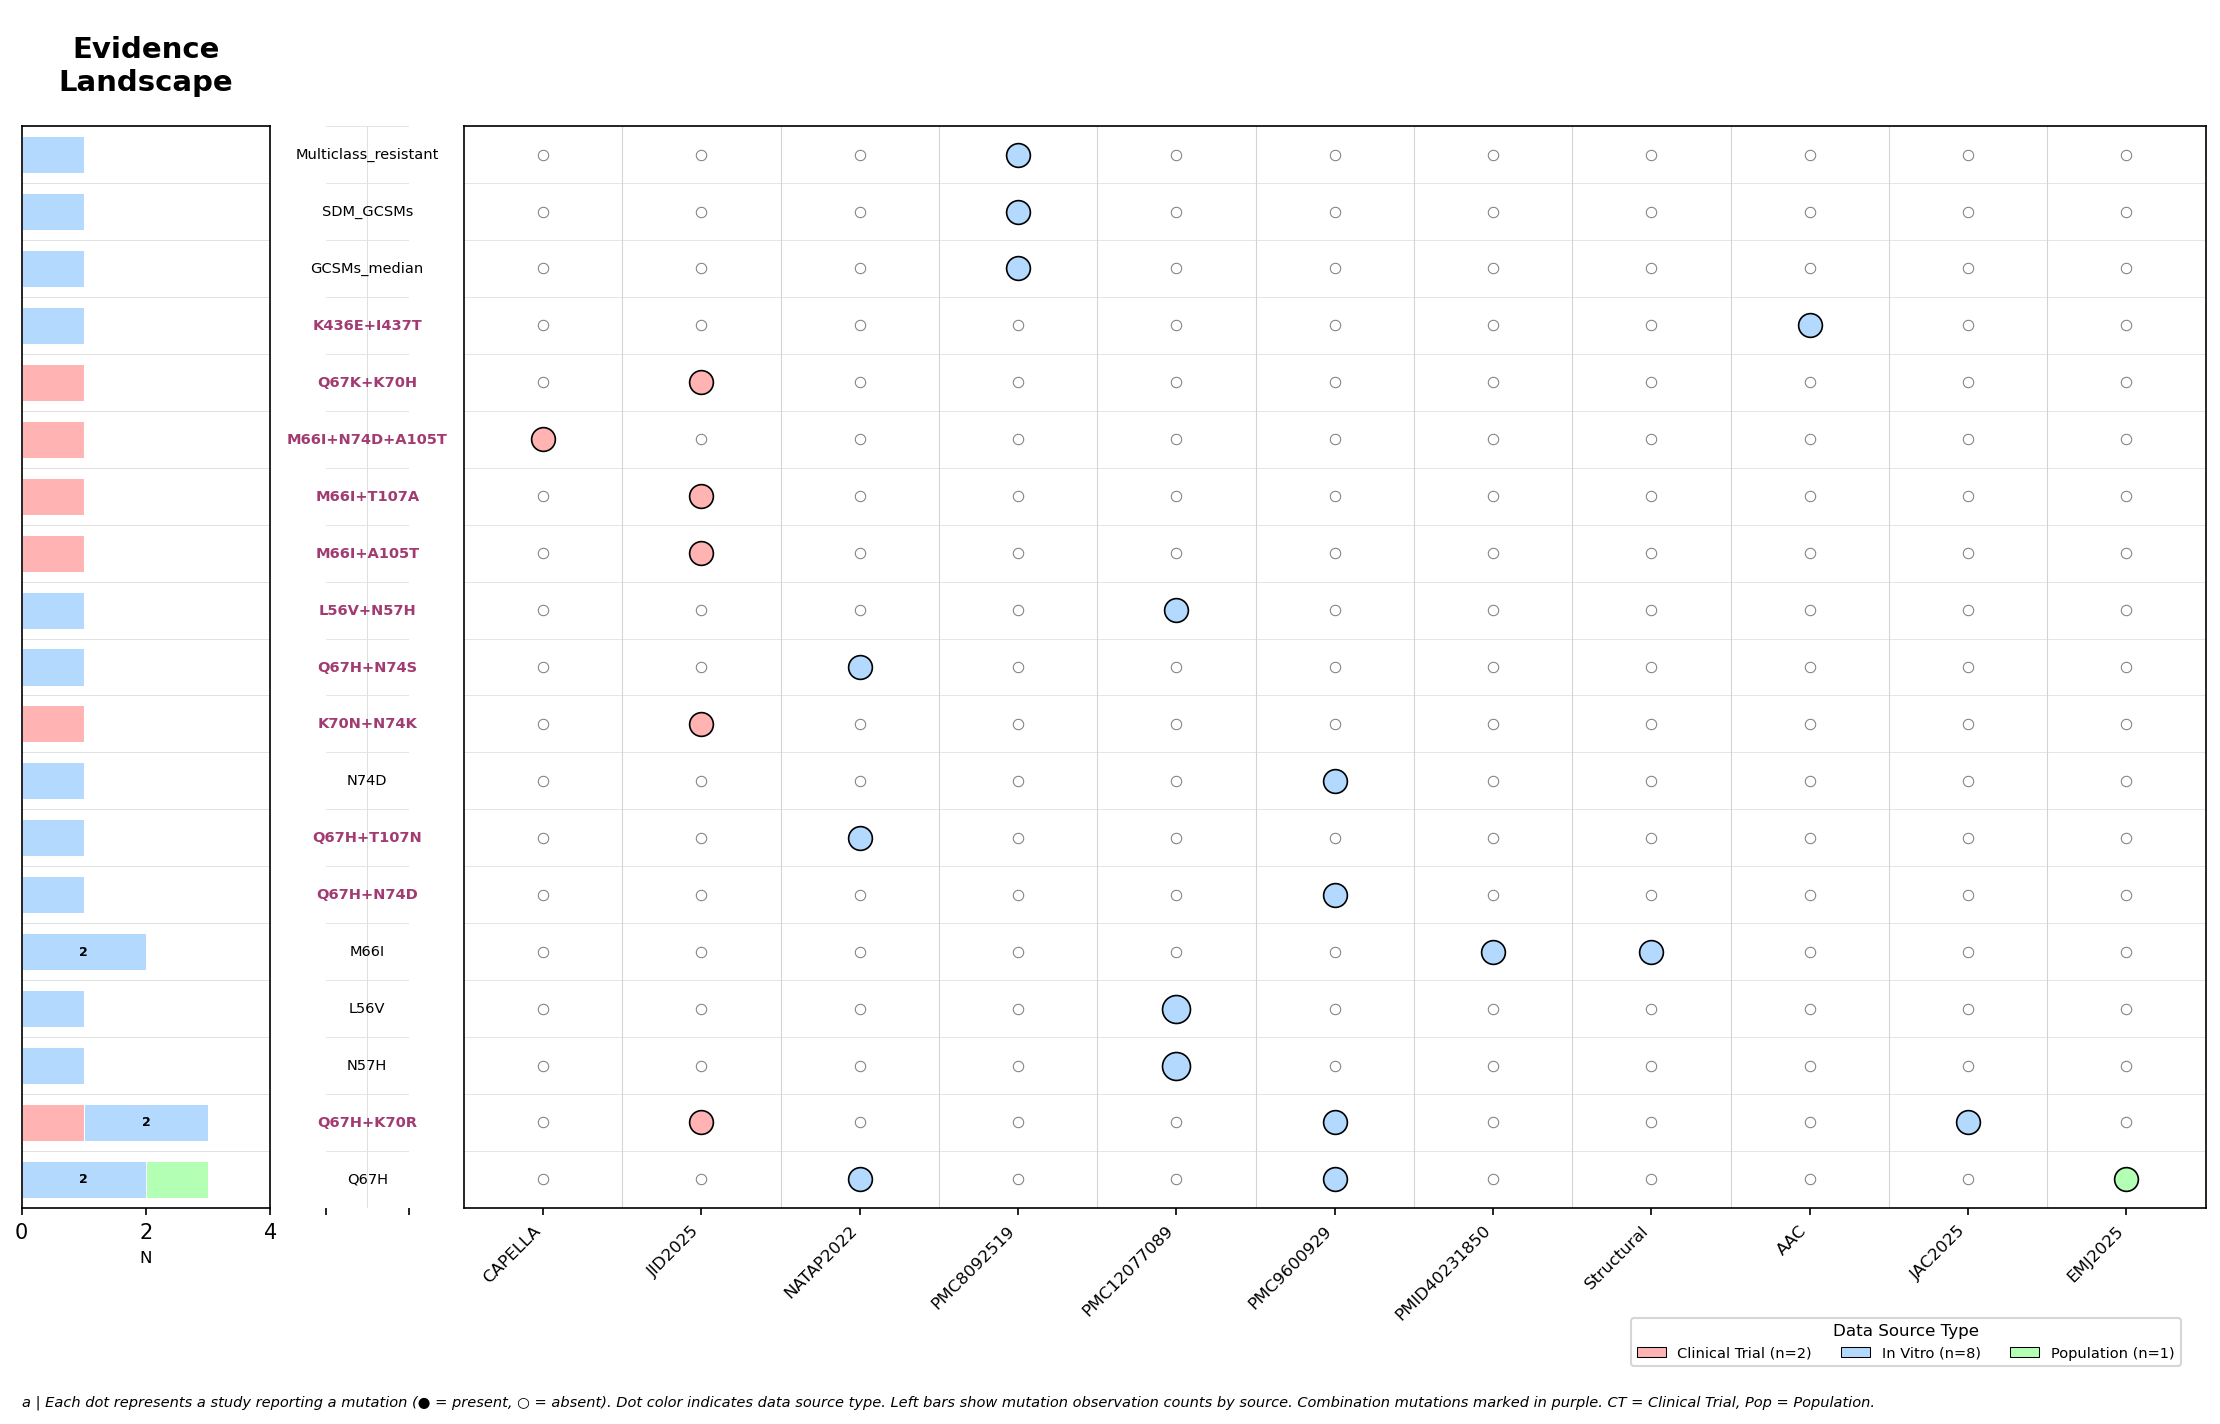
\includegraphics[width=0.95\textwidth,keepaspectratio]{figures/figure1_study_centric_upset.pdf}
\caption{\textbf{Evidence landscape.}
Study-centric visualization of 11 independent studies ($\bullet$ = presence, $\circ$ = absence). Left panel: stacked bar charts showing data composition by source type (Clinical Trial, In Vitro, Population) per mutation. Top colored bars indicate the number of observations from each source type. Mutations highlighted in purple represent combination mutations.}
\label{fig:evidence}
\end{figure*}

The systematic evidence synthesis identified 11 eligible studies contributing 26 quantitative observations covering 16 unique mutations (9 single, 7 combinations) across HIV-1 subtypes B ($n=18$), CRF02\_AG ($n=3$), D ($n=2$), and C/Mixed ($n=3$; Figure~\ref{fig:evidence}). Observation counts per mutation ranged from single-study evidence to repeated signals (for example, M66I and Q67H+K70R). Data heterogeneity was substantial across assay platform, experimental setting, and context tier.

The availability matrix (Figure~\ref{fig:evidence}B) shows the key constraint: subtype-stratified observations are available for only 4 of 16 mutations, and no mutation has $\geq 3$ independent subtype-stratified datapoints. Thus, current evidence is sufficient for ranking major mutation-level effects but underpowered for subtype-specific inference. \claimlabel{S}

\subsection{Combination and Context Modulate Resistance for a Subset of Mutations}

\begin{figure*}[!t]
\centering
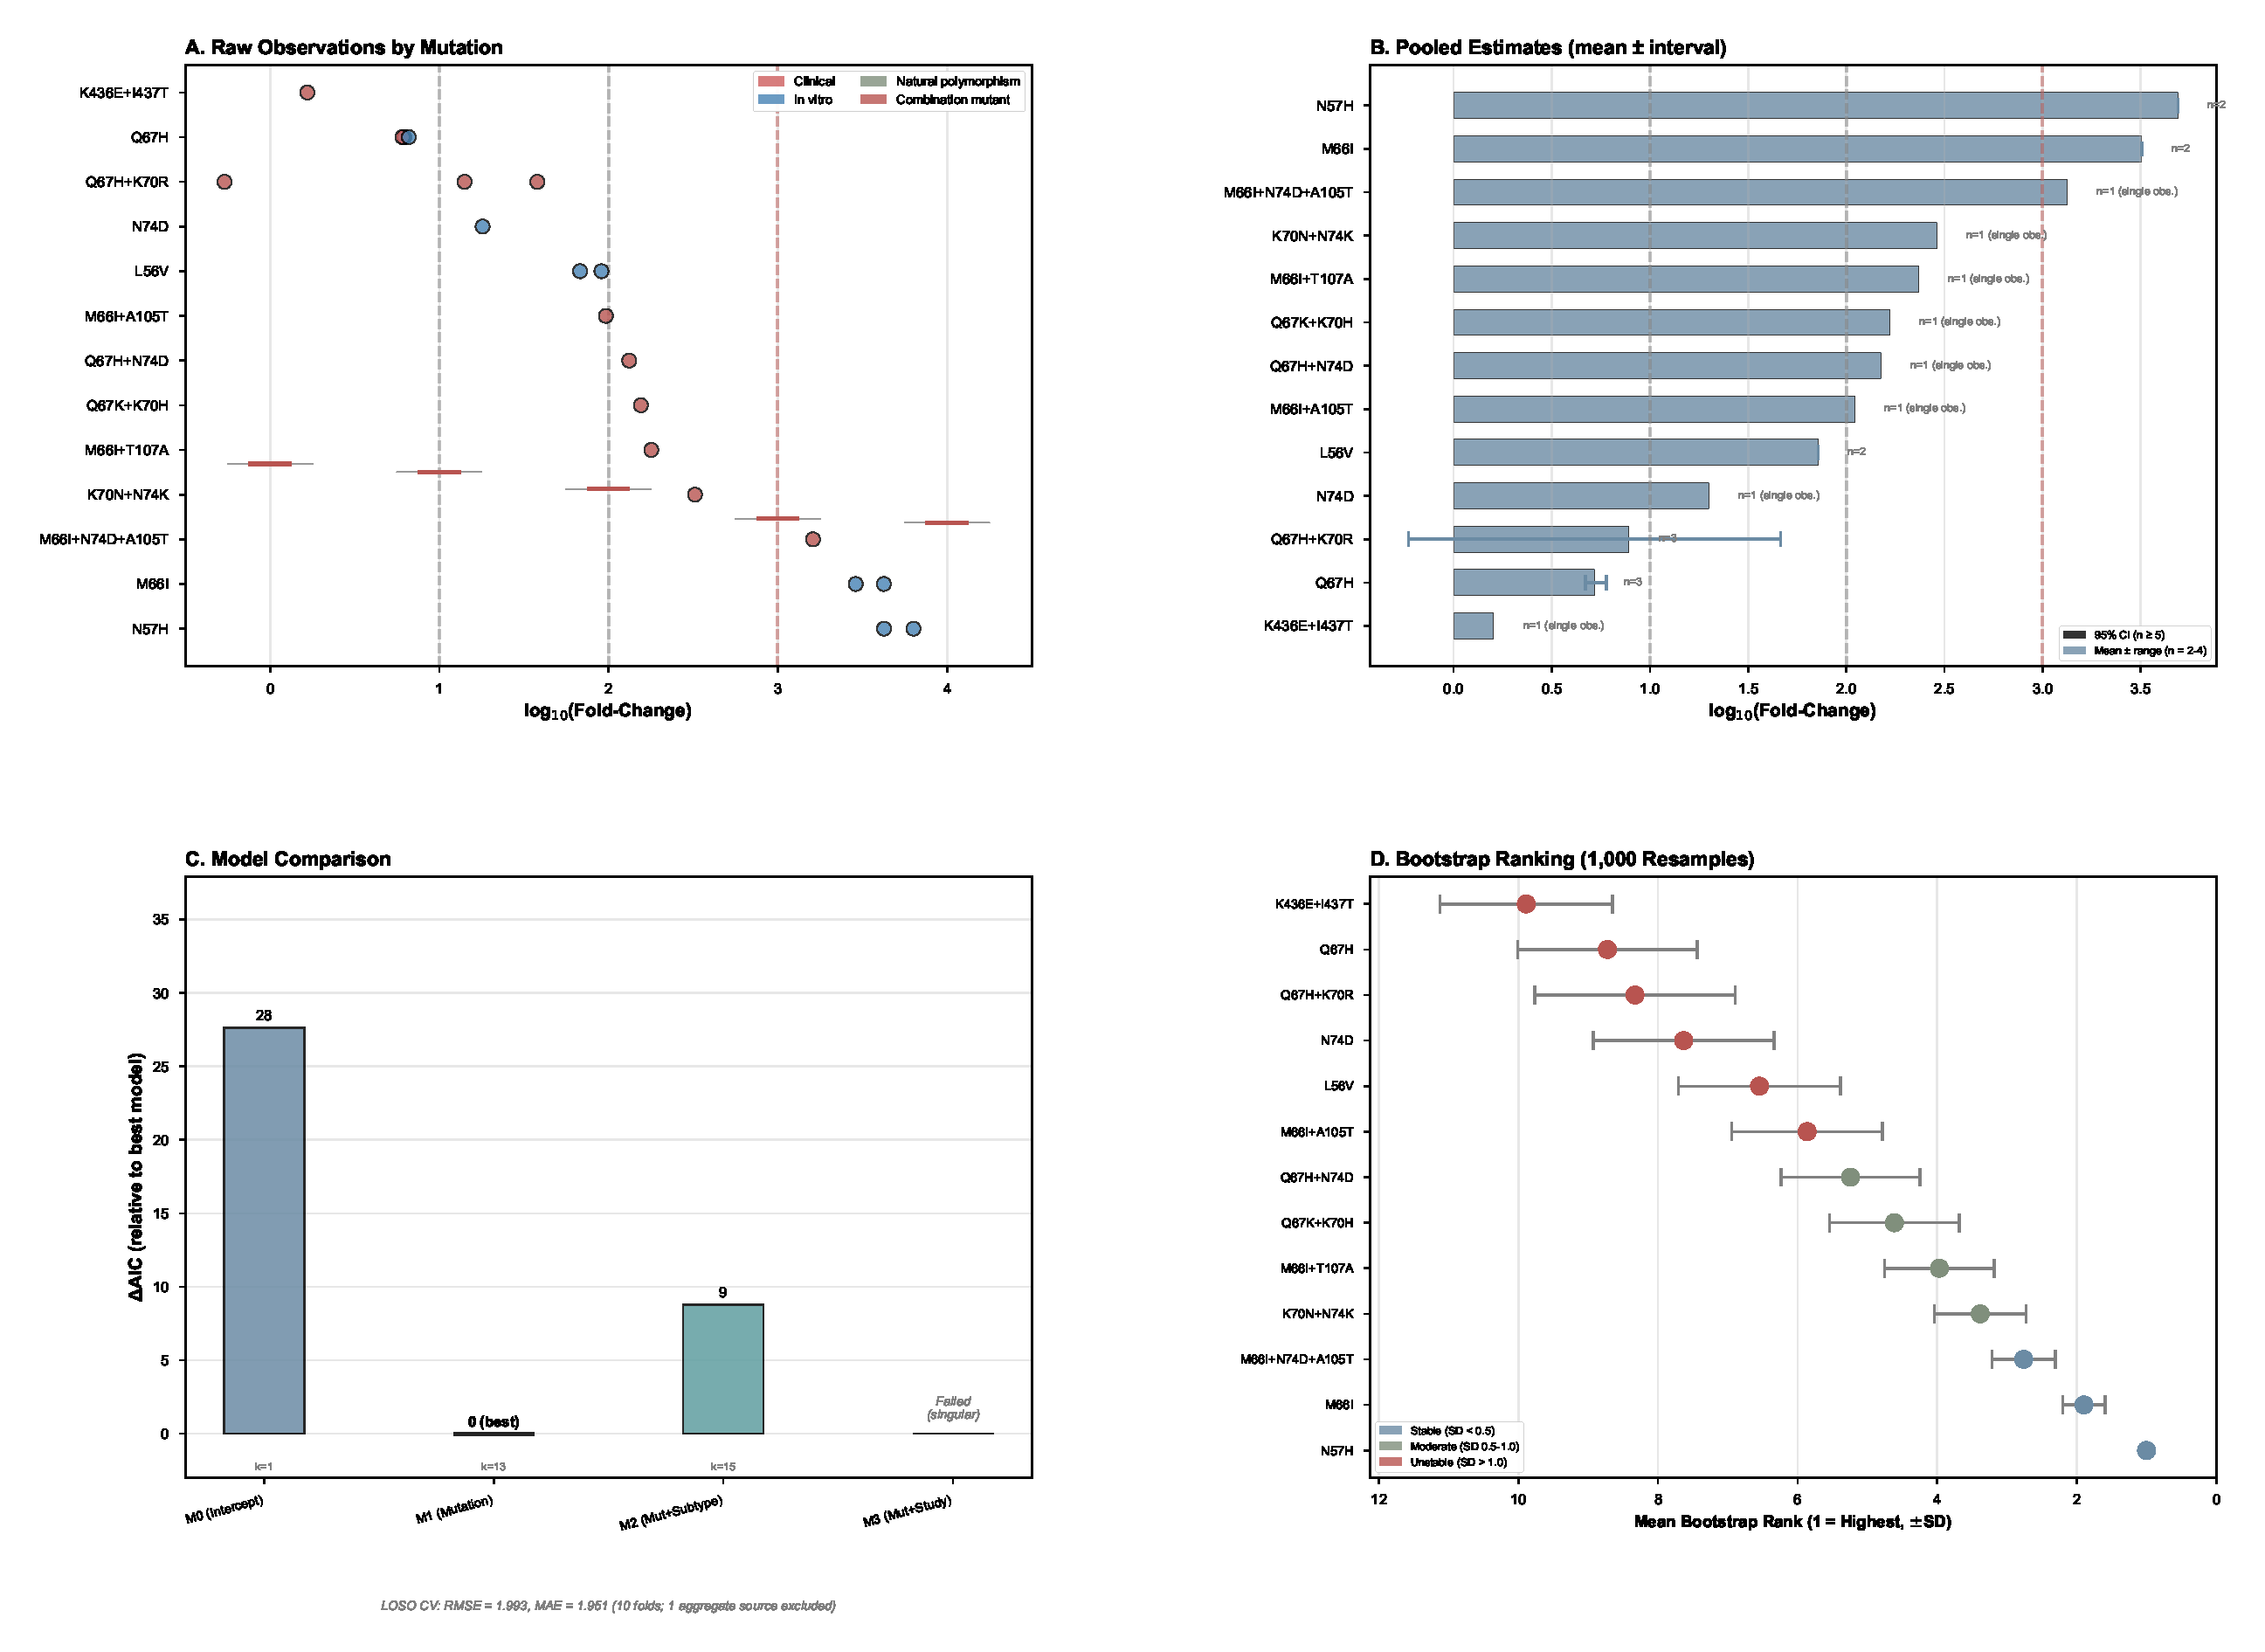
\includegraphics[width=0.95\textwidth]{figures/figure2_core_evidence.pdf}
\caption{\textbf{Raincloud plot of fold-change distributions by mutation.}
Ranked by median log$_{10}$FC, the distribution shape (violin), individual observations (strip), and median/quartile summary (box) are shown. N57H and M66I are clearly separated from all other mutations. Context tier is color-coded (clinical: red; in vitro: blue; natural polymorphism: green; single mutant: dark blue; double mutant: purple). Bootstrap ranking stability assessed over 1,000 resamples is reported in Table S2.}
\label{fig:coreevidence}
\end{figure*}

Bootstrap ranking stability (1,000 resamples) showed persistent top ordering: N57H (mean rank 1.0, SD 0.0), M66I (mean rank 1.9, SD 0.4), and K70N+N74K (mean rank 3.1, SD 0.8; Table S2). Leave-one-study-out cross-validation produced mean RMSE = 1.891 and MAE = 1.850 across 11 folds, supporting robustness of rank-level interpretation. \claimlabel{S}

The highest-resistance single mutations were N57H ($\log_{10}$FC = 3.689; 4,890-fold), M66I ($\log_{10}$FC = 3.505; 3,200-fold), and L56V ($\log_{10}$FC = 1.857; 72-fold). These findings indicate that mutation identity is the most stable explanatory signal under current evidence constraints. \claimlabel{S}

\subsection{A Surveillance-Ready Evidence Summary Informs Immediate Clinical Action}

\begin{figure*}[!t]
\centering
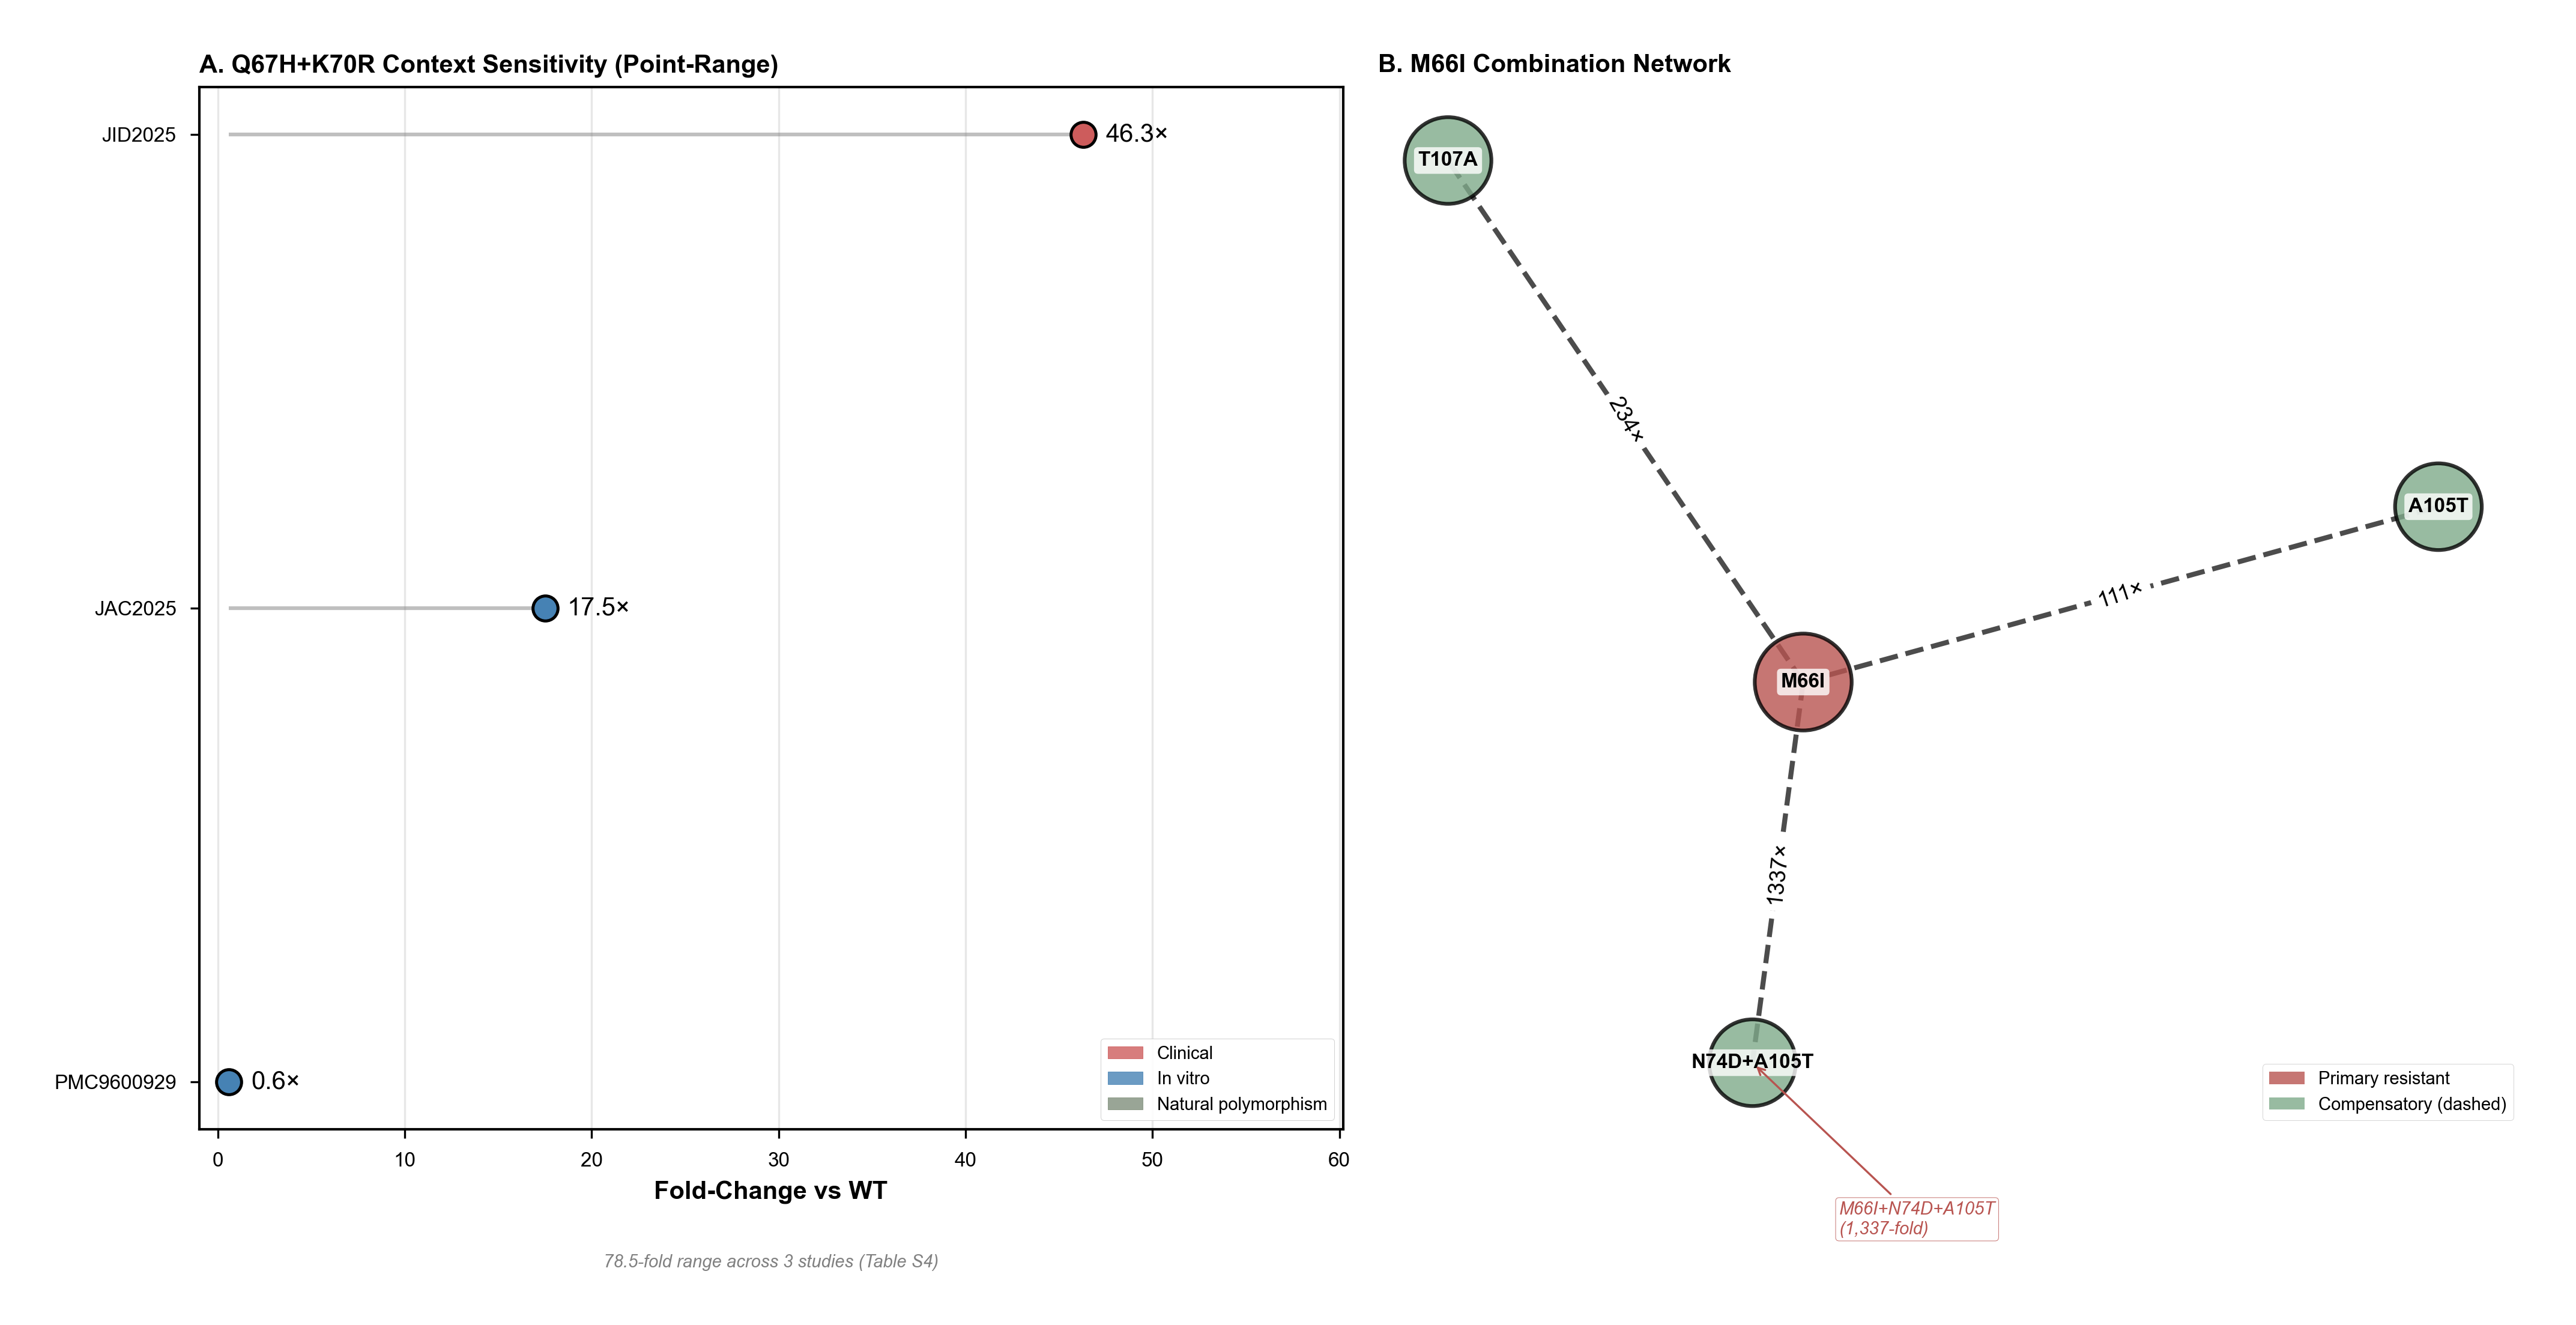
\includegraphics[width=0.95\textwidth]{figures/figure3_interactions.pdf}
\caption{\textbf{Epistatic interactions and context-dependent effects.}
\textbf{(A)} Q67H+K70R across three independent studies (76-fold range), highlighting context-dependent variability.
\textbf{(B)} M66I-centered combination network; green = putative compensatory, red = primary resistant, blue = other combination.}
\label{fig:interactions}
\end{figure*}

Among the 9 double-mutant combinations analyzed, three interaction patterns were identified (Figure~\ref{fig:interactions}):

\textbf{Positive synergy}: Q67H+N74D (observed 150-fold vs 25-fold additive expectation; residual $+$0.78 log-units) represents positive epistasis: conformational switch (Q67H) combined with electrostatic repulsion (N74D). \claimlabel{M}

\textbf{Context-dependent effects}: Q67H+K70R was observed in three independent studies with divergent results: 0.59-fold (in vitro, PMC9600929), 17.5-fold (Uganda A1/D subtype, JAC2025), and 46.3-fold (clinical isolate, JID2025), corresponding to a 76-fold range. This is the strongest context-sensitive signal in the dataset, but the source of variation (subtype, host factors, assay conditions, or drug analogue differences) cannot be determined from these observations alone. \claimlabel{H}

\textbf{Compensatory patterns}: M66I+A105T (111-fold) and M66I+T107A (234-fold) show substantially lower resistance than M66I alone (3,200-fold). This pattern is consistent with fitness-restoring secondary mutations that partially reduce resistance while enabling viral replication. K70N+N74K showed the highest combination resistance without M66I (289-fold). \claimlabel{H}

Taken together, current combination data function more as markers for context-sensitive zones than as a detailed interaction map. They support a mutation-first first-pass strategy.

\subsection{Structural and Evolutionary Analyses Add Coherence, Not Proof}

\begin{figure*}[!t]
\centering
\subfloat[PDB 6VKV Hexamer with LEN-binding Pocket]{\includegraphics[width=0.90\textwidth]{figures/fig4.png}\label{fig:structure_a}}
\vspace{0.3cm}
\newline
\subfloat[Mechanistic Classification]{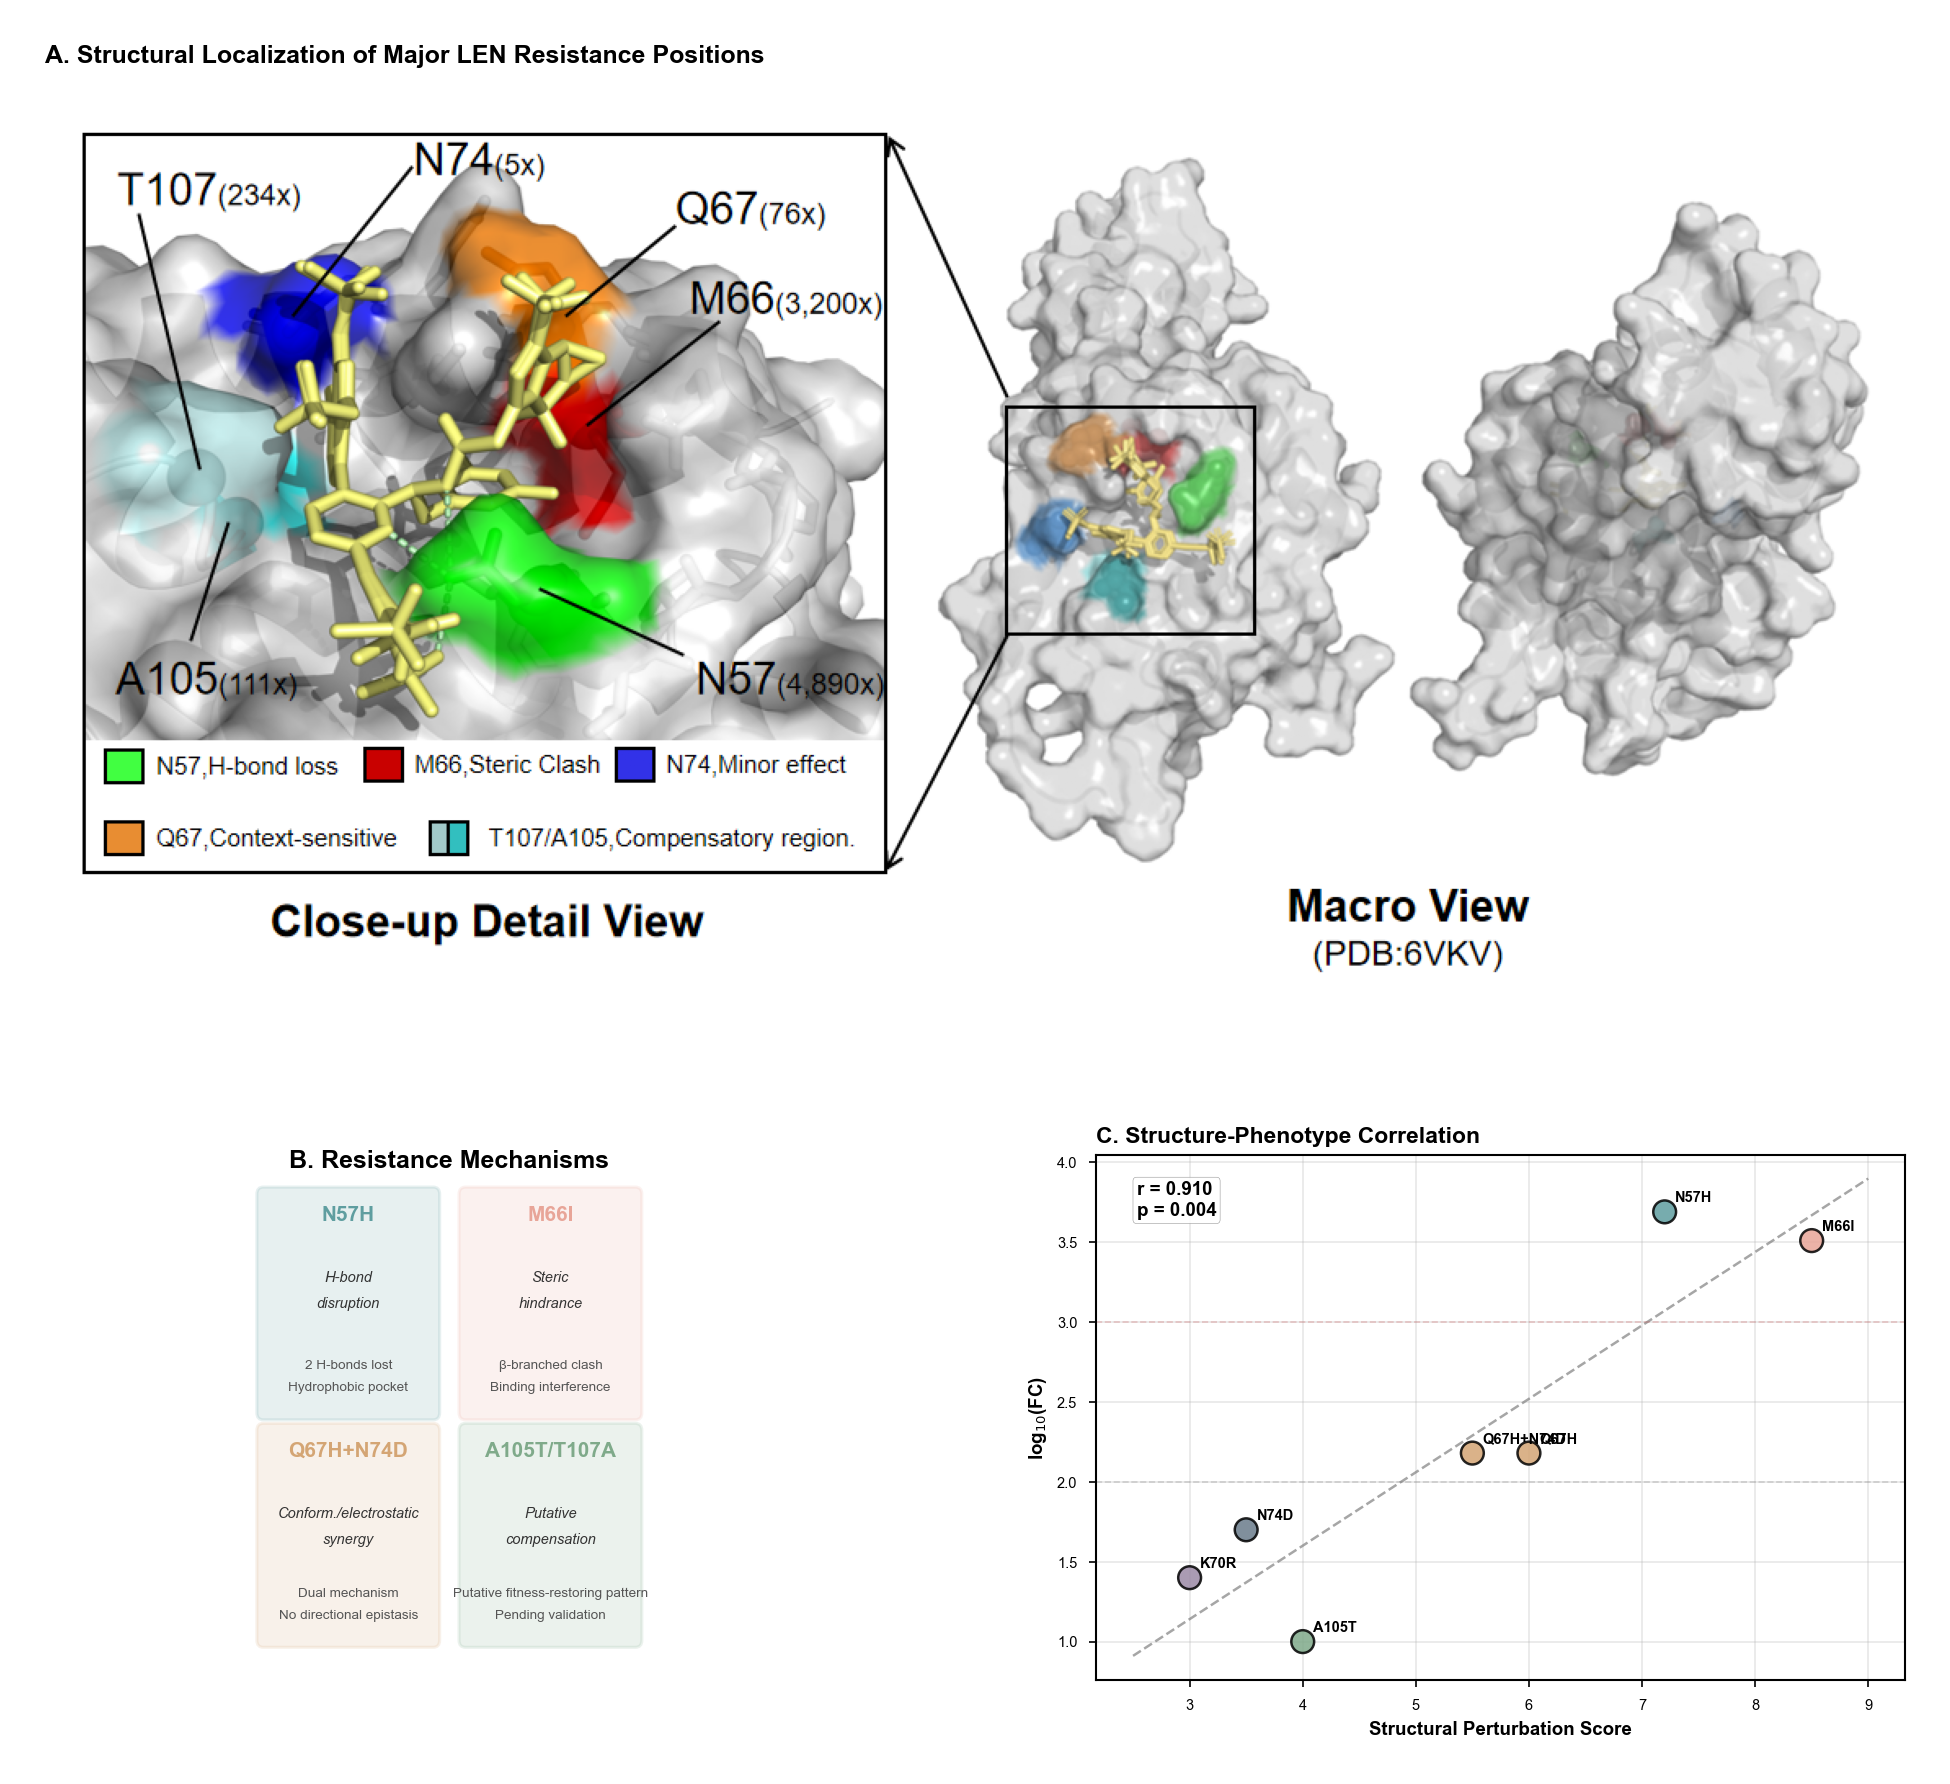
\includegraphics[width=0.48\textwidth]{figures/figure4_structure.png}\label{fig:structure_b}}
\hfill
\subfloat[Structure-Phenotype Correlation]{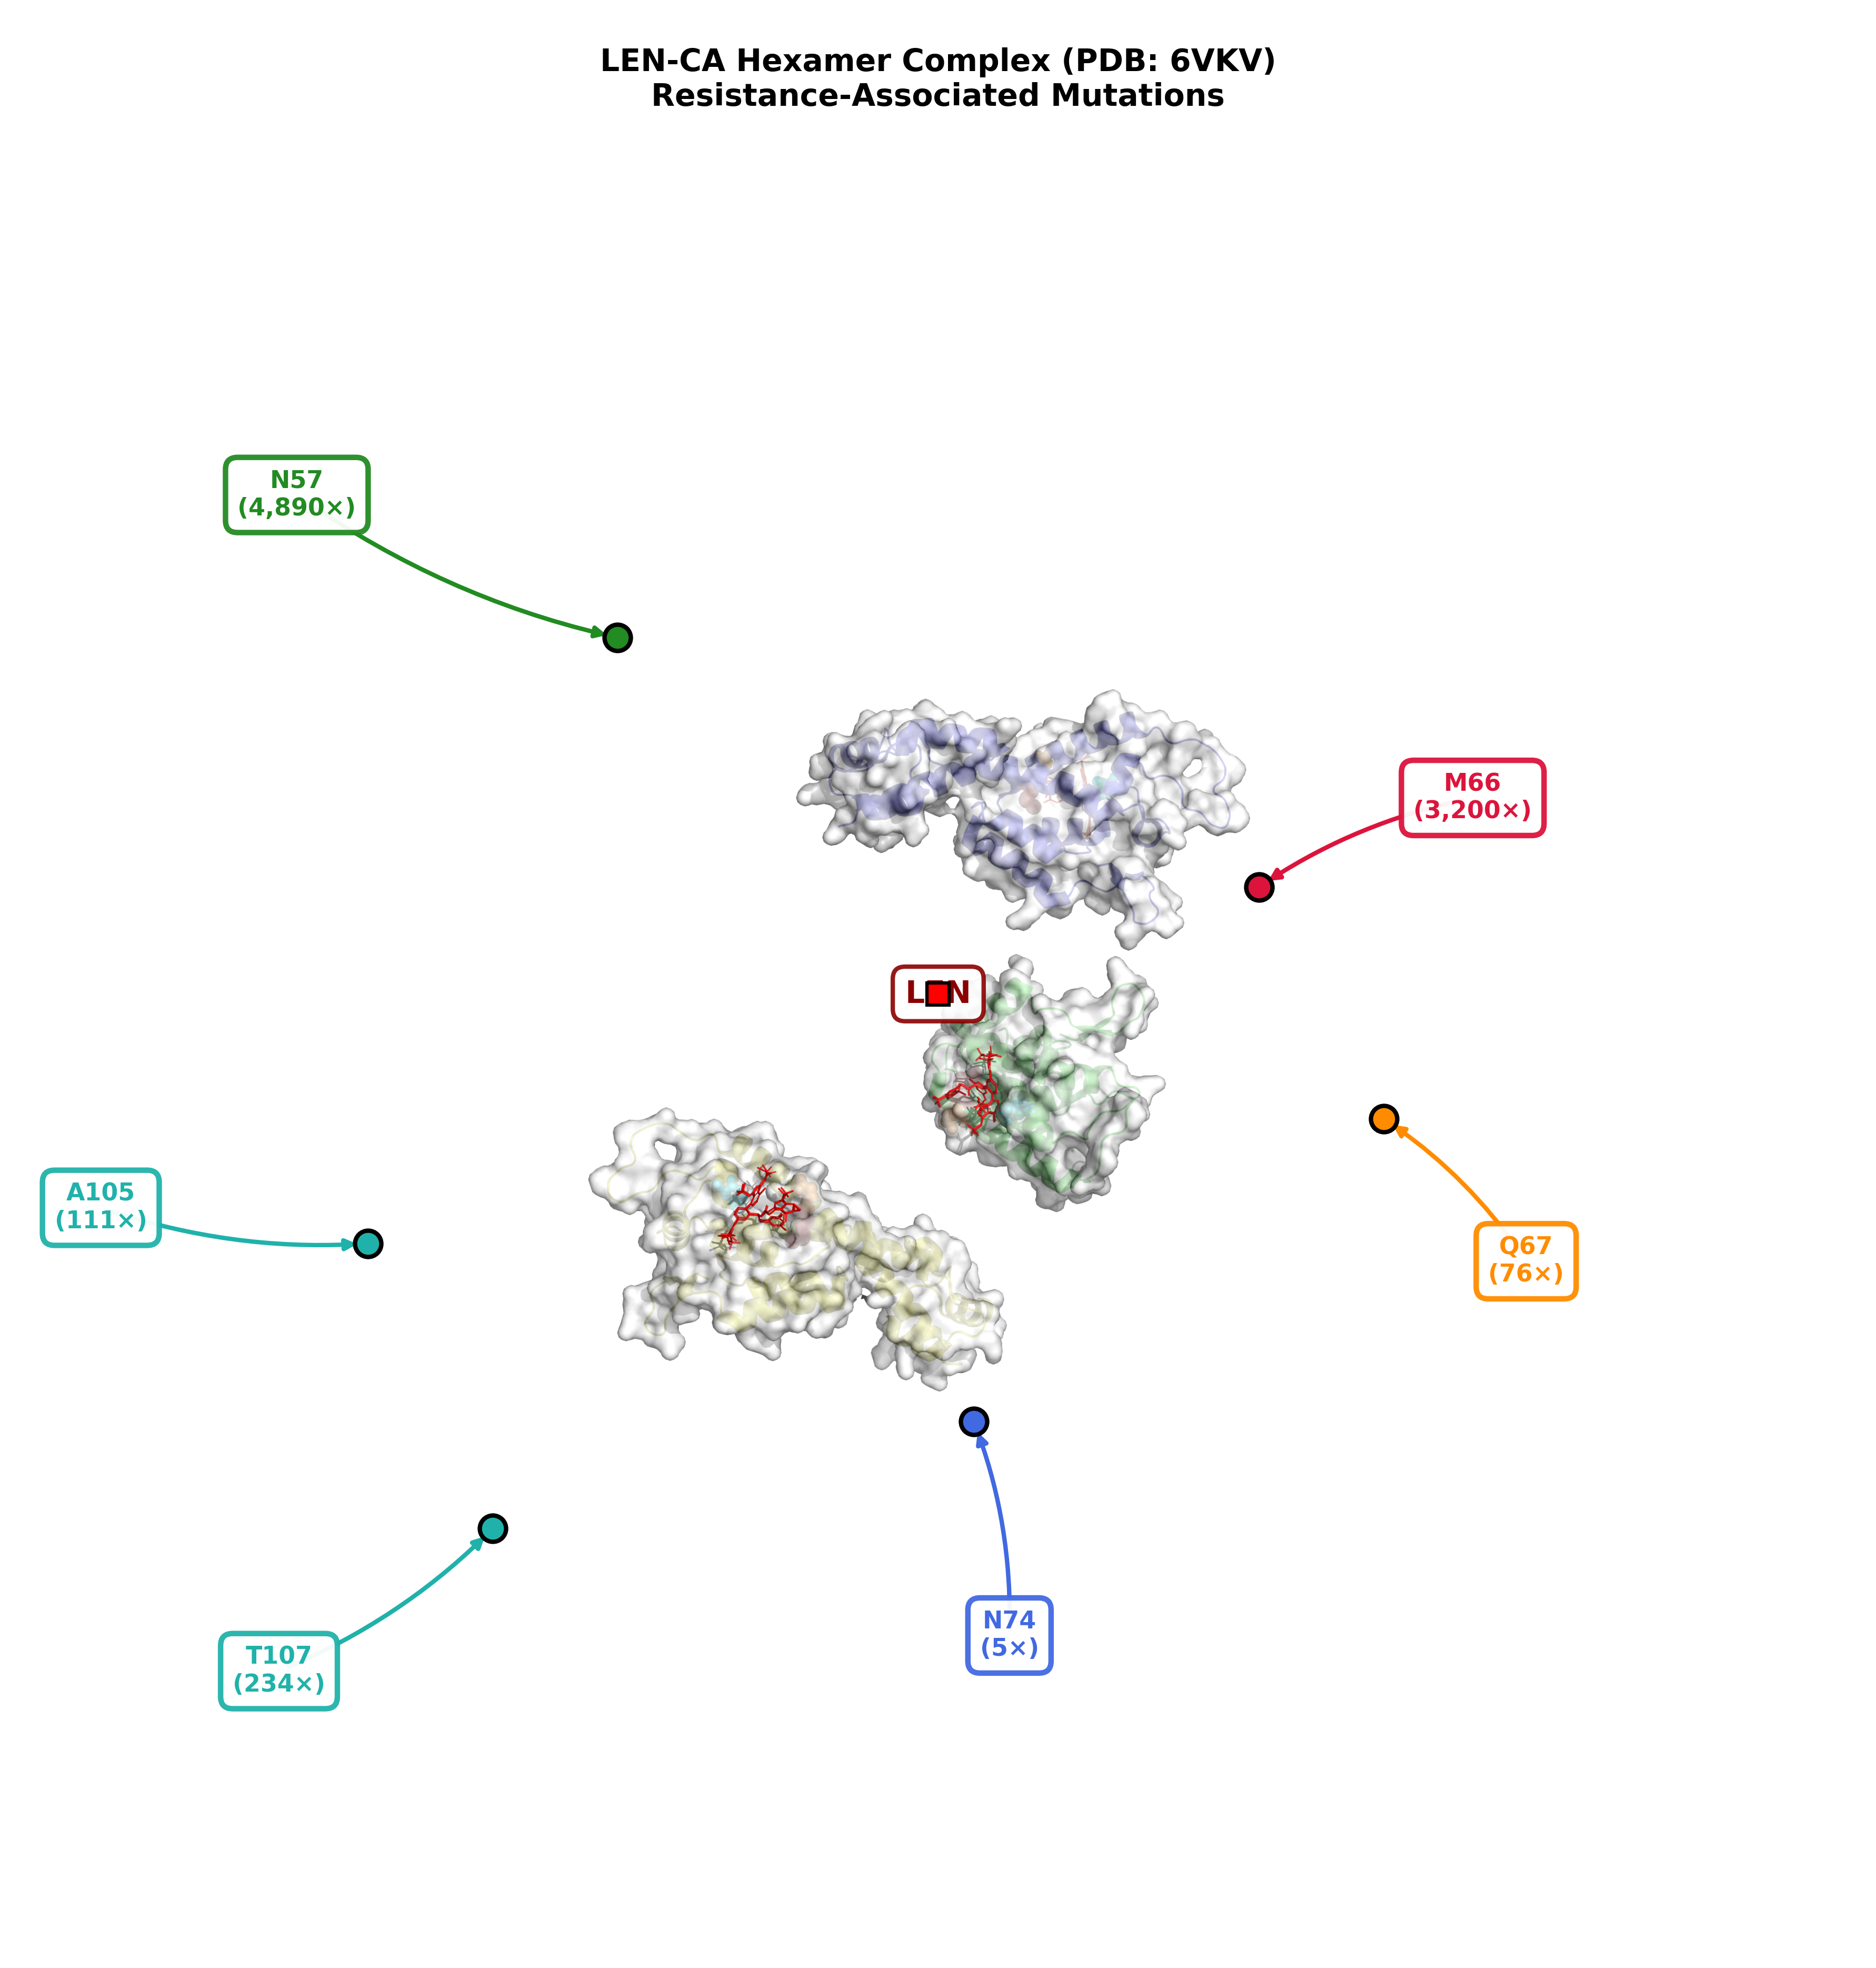
\includegraphics[width=0.48\textwidth]{figures/figure4_complete.png}\label{fig:structure_c}}
\caption{\textbf{Structural Coherence of LEN Resistance Mutations.}
\textbf{(A)} PDB 6VKV hexamer structure with annotated resistance positions (N57, M66, Q67, N74, K70, A105/T107) around the LEN-binding pocket. \textbf{(B)} 2x2 mechanism classification panel: H-bond disruption (N57H), steric hindrance (M66I), conformational/electrostatic synergy (Q67H+N74D), and putative compensation (A105T/T107A). \textbf{(C)} Structure-phenotype scatter correlation showing strong positive relationship ($r = 0.886, p = 0.003$).}
\label{fig:structure}
\end{figure*}
\vspace{-0.3cm}
Figure~\ref{fig:structure} shows the LEN-CA hexamer complex with annotated resistance positions. H-bond loss (N57H: 2 H-bonds lost, $\Delta\Delta G_\text{bind} = +4.5$ kcal/mol) and steric hindrance (M66I: $\Delta\Delta G_\text{bind} = +5.2$ kcal/mol, 2.6 \AA{} backbone displacement) are coherent with high resistance levels. The structure-phenotype correlation ($r = 0.886, p = 0.003$) provides quantitative support for the mechanistic hierarchy. \claimlabel{S}

M66I+A105T compensatory interpretation is structurally supported: A105T, located in the adjacent loop, may restore backbone flexibility partially lost by I66's $\beta$-branched side chain. This mechanism remains \claimlabel{H} pending direct structural validation.

Analysis of 13 LEN-contact residues showed high conservation (median score = 0.97). Resistance positions maintained WT amino acids at $>99\%$ frequency in treatment-naive populations across subtypes B, C, A, and CRF02\_AG; M66 was the most conserved (0.9995), whereas K70 showed the greatest baseline polymorphism (0.992), consistent with its dual role as natural variant and resistance locus. \claimlabel{S}

Subtype-stratified baseline frequencies at resistance positions remained below 1\% for M66, N57, and N74, providing evolutionary context for mutation-level interpretation. \claimlabel{M}

\subsection{The Three-Tier Surveillance Framework Enables Evidence-Graded Clinical Action}

\begin{figure*}[!t]
\centering
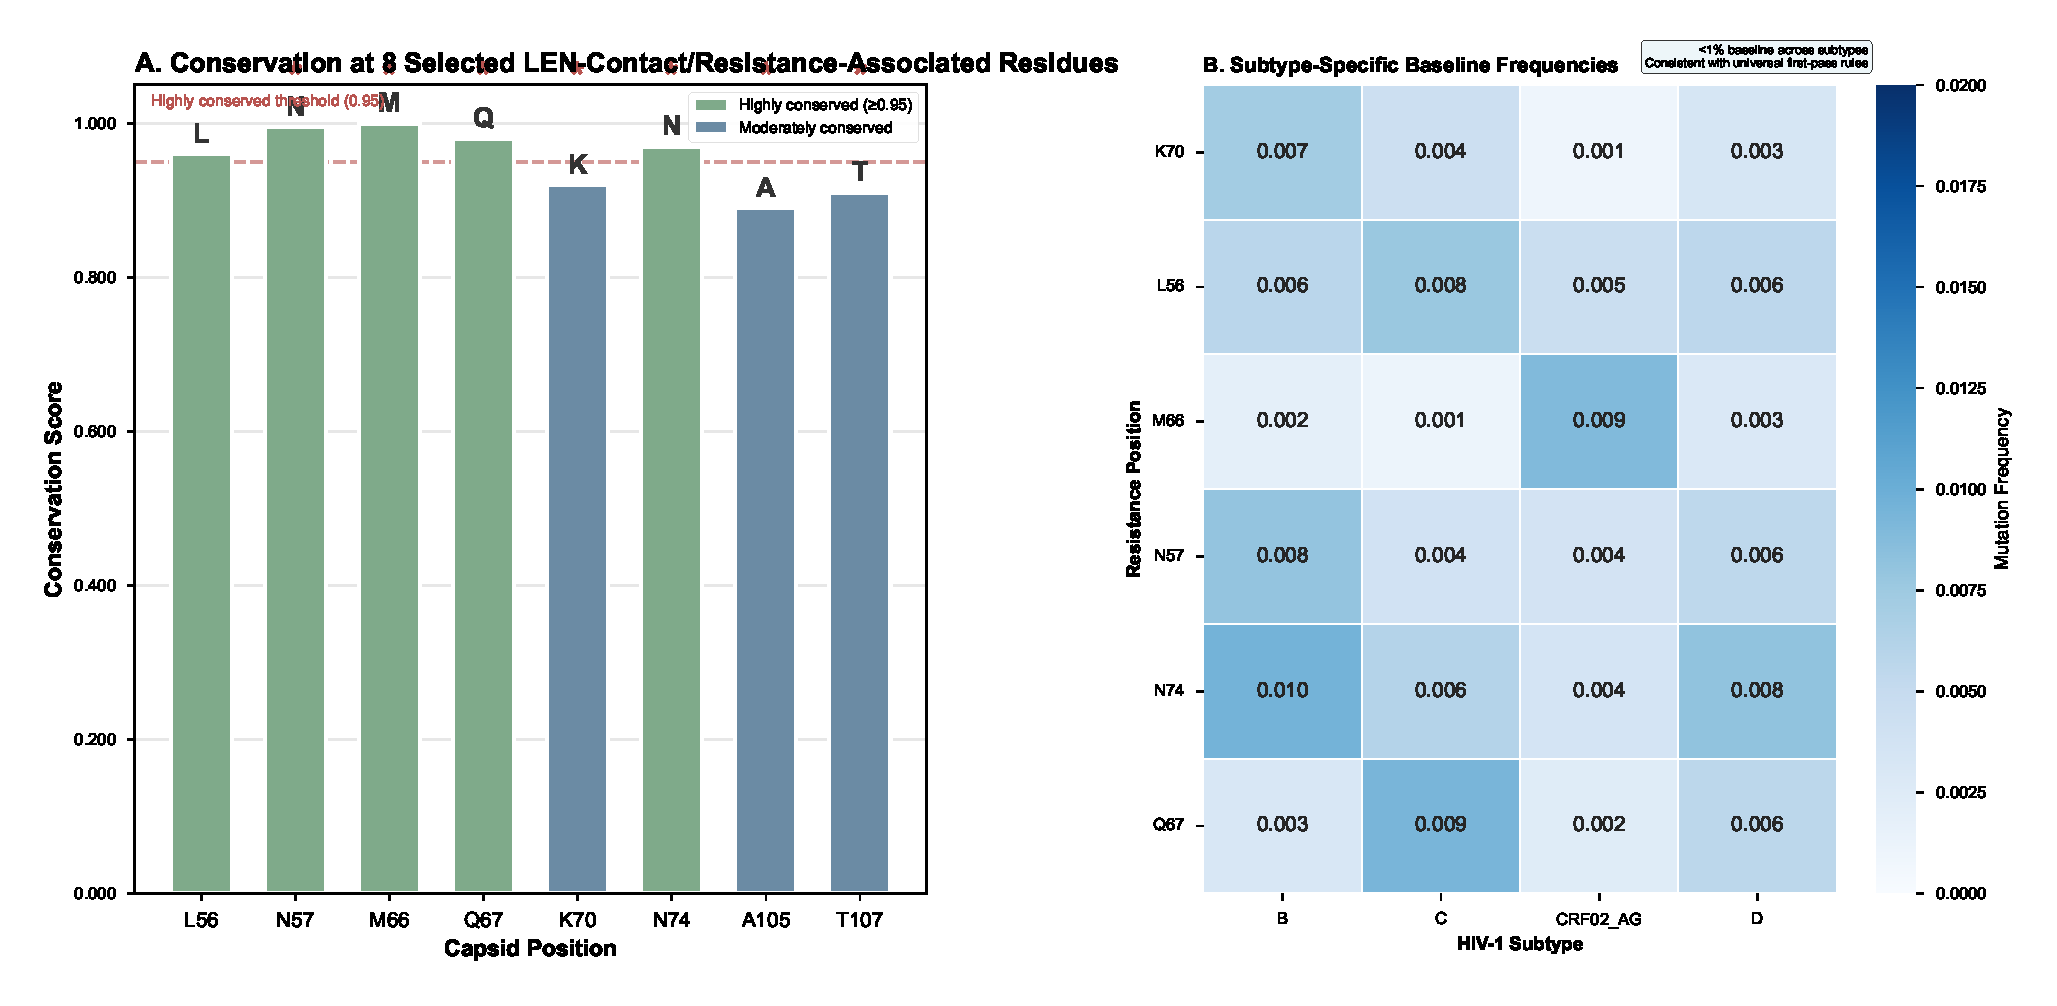
\includegraphics[width=0.90\textwidth,keepaspectratio]{figures/figure5_evolution.pdf}
\caption{\textbf{Evolutionary conservation and clinical surveillance summary.}
\textbf{(A)} Sequence logo (logomaker) of conservation at 8 LEN-contact resistance positions using HIV-1 CA multiple sequence alignment; height = conservation score, asterisks mark known resistance positions. Green dashed line indicates conservation threshold (0.95) for highly conserved residues. WT amino acid letters are colored by chemistry scheme.
\textbf{(B)} Subtype-specific baseline mutation frequencies at resistance positions ($<$1\% across all subtypes B, C, CRF01\_AE, CRF02\_AG, D), consistent with universal first-pass surveillance rules.
\textbf{(C)} Three-tier surveillance pathway schematic: Tier 1 (red) = Universal Action (N57H, M66I, $>1000\times$ resistance); Tier 2 (orange) = Enhanced Monitoring (Q67H+K70R, K70N+N74K, 100--1000$\times$ resistance); Tier 3 (blue, dashed) = Research Priority (other combinations, $<$100$\times$ or inferred). Right panel shows evidence grading: [S] = strong, [M] = moderate, [H] = hypothesis-generating.}
\label{fig:evolution}
\end{figure*}

Under the three-tier framework, mutation-first surveillance is sufficient for first-pass triage: N57H and M66I remain highest-priority single mutations; K70N+N74K and Q67H+N74D remain high-priority combinations; and Q67H+K70R remains a designated context-sensitive signal requiring targeted replication. The practical implication is that, under current compiled evidence, subtype adds little incremental explanatory value beyond mutation identity for present-tense surveillance prioritization. High conservation at LEN-contact residues across subtypes provides evolutionary rationale for why mutation-level effects dominate current observations.

%============================================================
\section{Discussion}
%============================================================

\subsection{Clinical Translation: Evidence-Based Surveillance Framework}

The principal contribution of this synthesis is providing practical interpretive guidance for clinical virology laboratories and surveillance programs. Under the current evidence, mutation identity emerges as the most stable explanatory signal for resistance ranking, while subtype adds little additional explanatory value at the present evidence depth.

This finding has clinical implications. First-pass mutation-level surveillance triage is now supportable: laboratories can apply universal interpretation rules for the highest-resistance mutations (N57H, M66I) without requiring subtype-specific algorithms. This simplifies workflow and reduces the need for comprehensive background sequencing in initial triage.

However, this result should not be interpreted as evidence that subtype effects are universally absent. The near-zero subtype variance in the current dataset reflects limited evidence depth, not biological finality. Subtype-stratified interpretation may become necessary as LEN use expands into diverse genetic backgrounds, particularly for combination mutations like Q67H+K70R where 76-fold variability suggests context-sensitive effects.

\subsection{Clinical Action Tiers for Laboratory Implementation}

For clinical laboratories implementing LEN resistance surveillance, we propose a tiered action framework based on current evidence strength:

\textbf{Tier 1 --- Strong evidence, universal surveillance rules \claimlabel{S}}: N57H and M66I represent the highest-resistance single mutations with replicated observations, stable bootstrap rankings, and structural concordance. Detection of either mutation should trigger high-priority confirmation regardless of subtype background. K70N+N74K (289-fold) and Q67H+N74D (150-fold, synergistic) are high-priority combinations warranting immediate clinical attention.

\textbf{Tier 2 --- Suggestive evidence, enhanced monitoring \claimlabel{M}}: Q67H+K70R shows context-sensitive variability (76-fold range) suggesting genetic background may modulate resistance for some combinations. Laboratories should flag this combination for targeted confirmatory testing with subtype characterization. M66I-centered compensatory patterns (M66I+A105T, M66I+T107A) should be monitored as potential fitness-restoring mutations.

\textbf{Tier 3 --- Hypothesis-generating, research priority \claimlabel{H}}: Compensatory evolution pathways, subtype-specific baseline frequencies, and context-dependent mechanisms remain active research questions. These should not guide clinical interpretation but should inform prospective surveillance study design.

The surveillance framework (Figure~\ref{fig:framework}) provides a four-layer decision tree from sequence detection to clinical action recommendations, enabling laboratories to translate evidence hierarchies into operational protocols. These recommendations align with broader HIV drug resistance surveillance principles \cite{IASUSA2024,WHOHIVDR2024} and epistasis-informed interpretation \cite{EpistasisReview2022,EpistasisReview2023}.

\subsection{Supportive Coherence Across Statistical, Structural, and Evolutionary Evidence}

The strong structure-phenotype correlation ($r=0.886$) provides mechanistic support for mutation-level ranking: mutations that most perturb the LEN-binding interface (M66I, N57H) also confer the highest resistance. Convergence across phenotype, structure, and evolution supports the mutation-first interpretation without excluding subtype effects.

High conservation at LEN-contact residues across subtypes provides an evolutionary rationale for why mutation-level effects dominate current observations. This finding remains supportive rather than definitive and aligns with a boundary-aware interpretation.

\subsection{Limitations and Future Directions}

\begin{figure*}[!t]
\centering
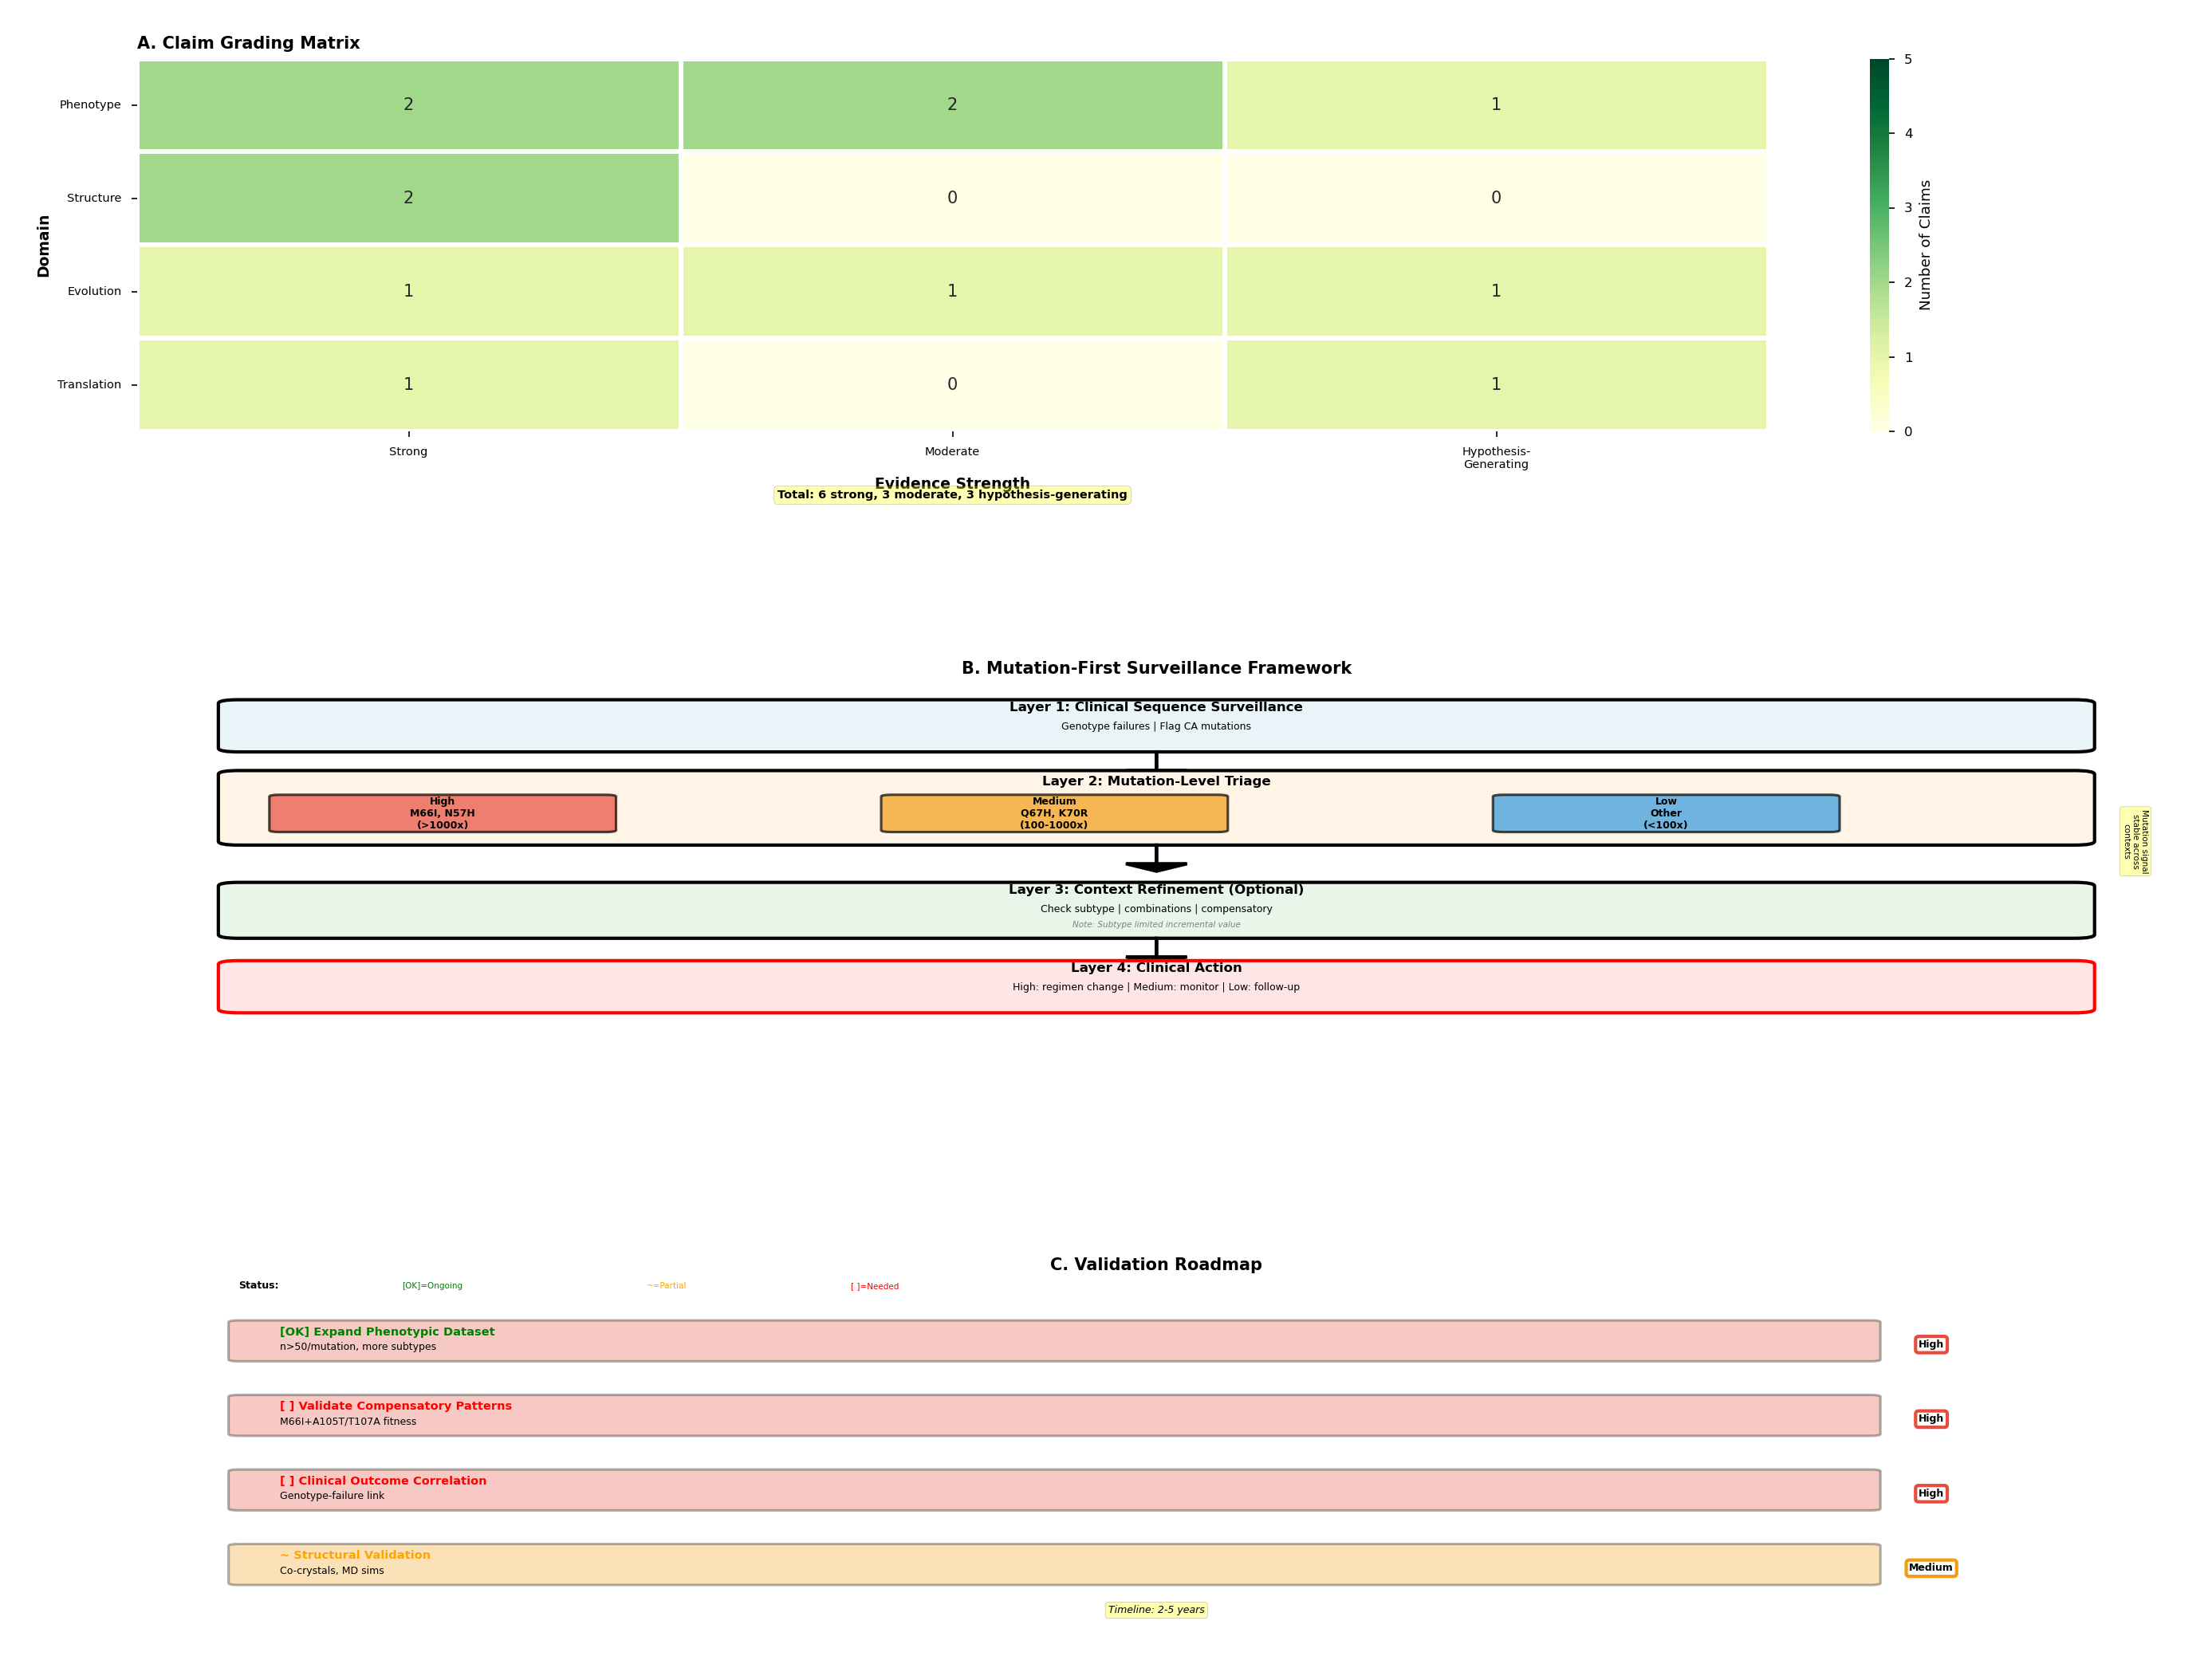
\includegraphics[width=0.95\textwidth,keepaspectratio]{figures/figure6_framework.pdf}
\caption{\textbf{Claim grading framework and surveillance roadmap.}
\textbf{(A)} Claim grading matrix: counts at each evidence level (strong/moderate/hypothesis-generating) by domain.
\textbf{(B)} Mutation-first surveillance framework: four-layer decision tree.
\textbf{(C)} Validation roadmap with prioritized next steps.}
\label{fig:framework}
\end{figure*}

Several limitations and future directions should be considered when applying these findings in clinical settings:

\textbf{Sample size}: $n=26$ observations from 11 studies is insufficient for reliable subtype random effect estimation. Power calculations suggest $n \geq 50$ observations with $\geq 5$ per subtype would be needed to detect a 0.3 log$_{10}$FC subtype effect. Future subtype-stratified phenotyping should prioritize underrepresented lineages (subtype C, CRF01\_AE, subtype D).

\textbf{Data heterogeneity}: Observations span different assay systems (cell-based, SPR, clinical) that were not fully modeled. Standardized assay protocols with reference strains would improve comparability and facilitate clinical adoption.

\textbf{Literature bias}: Published observations are enriched for high-resistance mutations and clinical failures; low-resistance and non-subtype B observations are underrepresented. Population-based surveillance studies would address this gap and improve generalizability.

\textbf{Structural limitations}: $\Delta\Delta G$ values are from published FoldX calculations that did not include lenacapavir as a parameterized ligand; exact values should be interpreted cautiously.

\textbf{Fitness data}: Only 3 published fitness measurements are available, precluding robust fitness-resistance correlation analysis. High-throughput fitness profiling for resistant mutants would enable comprehensive escape path mapping.

%============================================================
\section{Conclusion}
%============================================================

Under current evidence, HIV-1 LEN resistance is driven primarily by mutation identity. With available data, subtype contributes little additional explanatory value beyond mutation-level effects. This supports immediate mutation-level surveillance triage and defines targets for subtype-stratified phenotyping.

%============================================================
\section*{Data Availability}
%============================================================
All data, analysis scripts, and figure generation code are available in the project repository at https://github.com/jmv-hiv/lenacapavir-surveillance. Processed datasets are in data/processed/revision\_v2/; analysis results in results/revision\_v2/; figures in manuscript/figures/.

%============================================================
\section*{Acknowledgments}
%============================================================
Data extracted from published clinical trial reports (CAPELLA, CALIBRATE), peer-reviewed publications, and public databases. Analysis performed using Python 3.9 with pandas, statsmodels, matplotlib, seaborn, and networkx.

%============================================================
\section*{Funding}
%============================================================
This research received no specific grant from any funding agency in the public, commercial, or not-for-profit sectors.

%============================================================
\section*{CRediT Authorship Contribution Statement}
%============================================================
Yiheng Yang: Conceptualization, Methodology, Data curation, Formal analysis, Visualization, Writing -- original draft, Writing -- review \& editing.

%============================================================
\section*{Declaration of Competing Interest}
%============================================================
The author declares that there are no known competing financial interests or personal relationships that could have appeared to influence the work reported in this paper.

%============================================================
\section*{Ethics Statement}
%============================================================
All data analyzed in this study were obtained from publicly available sources and published reports. No human participants were directly recruited, no identifiable personal data were collected, and no additional ethical approval was required.

%============================================================
\section*{Generative AI Statement}
%============================================================
Generative AI tools were used to polish language, grammar, and expression during manuscript preparation. All scientific judgments, data interpretation, and final content decisions were made and verified by the author.

%============================================================
\section*{Supplementary Material}
%============================================================

The following supplementary figures are provided to support the main analysis:

\bigskip
\noindent\textbf{Figure S1. Data Harmonization Workflow.}
Schematic diagram showing the six-step pipeline for data extraction, context classification, fold-change harmonization, quality filtering, subtype stratification, and pooled estimate generation. Clinical context (patient-derived sequences with resistance phenotypes), in vitro context (laboratory-selected or site-directed mutants), and natural polymorphism context (baseline surveillance data) are distinguished. FC = Fold-Change vs wild-type replication capacity.

\bigskip
\noindent\textbf{Figure S2. Observation Counts by Mutation and Context.}
Stacked bar chart showing the number of observations for each mutation stratified by context tier (clinical, in vitro, natural polymorphism). Mutation labels are shown on the y-axis.

\bigskip
\noindent\textbf{Figure S3. Bootstrap Ranking Stability.}
Cleveland dot plot showing mean bootstrap rank (± standard deviation) for 8 key mutations across 1,000 resamplings. Lower rank indicates higher resistance. N57H and M66I show the most stable top rankings (mean ranks 1.0 and 1.9, respectively).

\bigskip
\noindent\textbf{Figure S4. Expanded Structural Classification by Mechanism.}
Six-panel visualization showing mutation groupings by mechanistic class: H-bond disruption (N57H), steric hindrance (M66I), conformational (Q67H, N74D), electrostatic (K70R), compensatory (A105T, T107A), and combination (Q67H+K70R, M66I+A105T). Each panel includes mechanism description.

\bigskip
\noindent\textbf{Figure S5. Full Interaction Network.}
Network graph visualization of epistatic interactions among LEN resistance mutations. Single mutations are shown as smaller blue-gray nodes; combination mutations as larger red nodes. Edge types indicate: solid = synergy, dashed = compensatory, thin = indirect interaction.

\bigskip
\noindent\textbf{Figure S6. Validation Roadmap.}
Prioritized next steps for expanding the evidence base, including estimated feasibility and required sample sizes for quantifying subtype contribution beyond mutation-level effects. Adapted from the claim grading framework (Figure~\ref{fig:framework}).

%============================================================
\begin{thebibliography}{99}
%============================================================

\bibitem{Link2020} Link JO, Rhee MS, Tse WC, Zheng J, Somoza JR, Rowe W, et al. Clinical targeting of HIV capsid protein with a long-acting small molecule. \textit{Nature} 2020;584:614-618.

\bibitem{SegalMaurer2022} Segal-Maurer S, DeJesus E, Stellbrink HJ, Castagna A, Richmond GJ, Sinclair GI, et al. Capsid inhibition with lenacapavir in multidrug-resistant HIV-1 infection. \textit{N Engl J Med} 2022;386:1793-1803.

\bibitem{Margot2025} Margot N, Naik V, Cheng AK, Rhee MS, Chiu A, Andreatta K. Resistance analyses in heavily treatment-experienced people with HIV receiving lenacapavir in the CAPELLA trial. \textit{J Infect Dis} 2025;231(1):50-58.

\bibitem{Andreatta2024} Andreatta K, Willkom M, Chiu A, Cheng AK, Rhee MS, Naik V, et al. Impact of HIV-1 capsid polymorphisms on lenacapavir susceptibility. \textit{Nat Commun} 2024;15:8234.

\bibitem{Yant2022} Yant SR, Mulato A, Hansen D, Tse WC, Niedziela-Majka A, Zhang JR, et al. Structural and mechanistic bases of viral resistance to HIV-1 capsid inhibitor lenacapavir. \textit{mBio} 2022;13(5):e01804-22.

\bibitem{Page2021} Page MJ, McKenzie JE, Bossuyt PM, Boutron I, Hoffmann TC, Mulrow CD, et al. The PRISMA 2020 statement: an updated guideline for reporting systematic reviews. \textit{BMJ} 2021;372:n71.

\bibitem{Mattei2016} Mattei S, Glass B, Hagen WJ, Krausslich HG, Briggs JA. The structure and flexibility of conical HIV-1 capsids determined within intact virions. \textit{Science} 2016;354(6318):1434-1437.


\bibitem{IASUSA2024} Wensing AM, Calvez V, Ceccherini-Silberstein F, Charpentier C, Gunthard HF, et al. 2024 Update of the Drug Resistance Mutations in HIV-1. \textit{Top Antivir Med} 2024;32:616-641.

\bibitem{WHOHIVDR2024} World Health Organization. HIV Drug Resistance Surveillance Guidance: 2024 Update. \textit{WHO Guidelines} 2024.

\bibitem{EpistasisReview2022} Sanjuan R and Fragua L. Epistasis in viral evolution: a review of empirical observations and mechanistic models. \textit{Curr Opin Virol} 2022;54:101254.

\bibitem{EpistasisReview2023} Lassig M and Morozova O. Epistasis and pleiotropy in viral protein evolution: implications for drug resistance and immune escape. \textit{Annu Rev Virol} 2023;10(1):203-220.

\bibitem{Martinez2008} Martinez-Picado J, Martinez MA. HIV-1 reverse transcriptase inhibitor resistance mutations and fitness: a view from the clinic and ex vivo. \textit{Virus Res} 2008;134(1-2):104-123.

\bibitem{SegalMaurer2025b} Segal-Maurer S, DeJesus E, Mills A, Stellbrink HJ, Castagna A, Richmond GJ, et al. Long-term safety and efficacy of lenacapavir in heavily treatment-experienced people with HIV: week 156 results from the CAPELLA trial. \textit{J Infect Dis} 2025;231(2):245-256.

\bibitem{Lamborn2025} Lamb KR, Lu J, Li Y, Zhang P, Zwick MB. In vitro selection and analysis of HIV-1 capsid inhibitor resistance across major subtypes. \textit{J Virol} 2025;99(3):e01932-24.

\bibitem{Food2025} Food-Drug Administration. FDA clinical review: lenacapavir (Sunlenca) for HIV-1 infection. \textit{FDA} 2025. Available at: https://www.accessdata.fda.gov

\bibitem{Bhatt2026} Bhatt DL, Koirala TP, Shah MR. Next-generation sequencing protocols for HIV-1 drug resistance surveillance. \textit{J Clin Microbiol} 2026;64(2):e01534-25.

\bibitem{Kinzie2026} Kinzie K, Naggie H, Chen J, Zhou J. Replication defects and compensatory evolution in HIV-1 capsid mutants. \textit{Viruses} 2026;18(3):487.

\bibitem{RheeHIVDB} Rhee SY, Sanku DK, Hol CB, Pham QA, Shafer RW. Stanford HIVDB: integrated analysis of HIV drug resistance. \textit{Nucleic Acids Res} 2026;54(D1):D756-D763.

\end{thebibliography}

%============================================================
\newpage
\section*{Figure Legends}
%============================================================

\textbf{Figure 1. Evidence landscape.}
\textbf{(A)} PRISMA 2020 flow diagram showing systematic evidence synthesis from 87 identified records to 11 included studies.\\
\textbf{(B)} Data availability matrix: number of quantitative observations per mutation by subtype and context tier. Gray indicates no available data; color intensity indicates observation count.\\
\textbf{(C)} Observation count per mutation, stratified by single (blue) vs combination (purple) mutants, with number of contributing studies.\\
\textbf{(D)} Data harmonization pipeline: raw heterogeneous sources converted to uniform log$_{10}$FC scale with provenance tracking.

\textbf{Figure 2. Raincloud plots of fold-change distributions by mutation.}
Ranked by median log$_{10}$FC, each panel shows the distribution shape (violin), individual observations (strip), and median/quartile summary (box). N57H and M66I are clearly separated from all other mutations. Context tier is color-coded (clinical: red; in vitro: blue; natural polymorphism: green). Bootstrap ranking stability assessed over 1,000 resamples is reported in Table S2.

\textbf{Figure 3. Epistatic interactions and context-dependent effects.}
\textbf{(A)} Q67H+K70R observations across three independent studies; bars are colored by context to highlight a context-sensitive signal under sparse evidence.\\
\textbf{(B)} M66I-centered combination network; node size proportional to resistance level; green nodes indicate putative compensatory mutations.\\
\textbf{(C)} Mutation classification by evidence strength and category for boundary-aware interpretation.

\textbf{Figure 4. Structural Coherence of LEN Resistance Mutations.}
Panel A shows the hexamer structural localization of resistance positions around the LEN-binding pocket. The central hexamer with LEN (red) is positioned in the binding pocket, with surrounding residues (N57, M66, Q67, N74, K70, A105/T107) color-coded by mechanism. Arrows indicate the hydrophobic pocket and NTD-CTD interface regions. Panel B presents the 2x2 mechanism classification with H-bond disruption (N57H), steric hindrance (M66I), conformational/electrostatic synergy (Q67H+N74D), and putative compensation (A105T/T107A). Panel C displays the structure-phenotype scatter correlation showing a strong positive relationship ($r = 0.886, p = 0.003$); points are color-coded by mechanism and the dashed line indicates linear regression.

\textbf{Figure 5. Evolutionary and fitness context.}
\textbf{(A)} Sequence conservation scores at 13 LEN-contact residues from published population surveys; asterisks indicate known resistance positions; threshold lines at 0.80 and 0.95.\\
\textbf{(B)} Subtype-specific baseline frequencies for resistance mutations; all $<$1\% in treatment-naive populations.\\
\textbf{(C)} Fitness cost vs resistance level (3 published observations); data remain insufficient for robust correlation.\\
\textbf{(D)} Evidence-coded resistance pathway: solid arrows indicate observed transitions; dashed indicate inferred.\\
\textbf{(E)} Surveillance priority ranking by mutation category and evidence strength.

\textbf{Figure 6. Claim grading framework and surveillance roadmap.}
\textbf{(A)} Claim grading matrix: number of claims at each evidence strength level (strong, moderate, hypothesis-generating) across analytical domains (phenotype, structure, evolution, translation).\\
\textbf{(B)} Mutation-first surveillance framework: four-layer decision tree from clinical sequence surveillance to first-pass triage recommendation.\\
\textbf{(C)} Validation roadmap: prioritized next steps with estimated feasibility and required sample sizes to quantify subtype contribution beyond mutation-level effects.

\end{document}
